% Options for packages loaded elsewhere
\PassOptionsToPackage{unicode}{hyperref}
\PassOptionsToPackage{hyphens}{url}
\PassOptionsToPackage{dvipsnames,svgnames,x11names}{xcolor}
%
\documentclass[
  12pt,
]{article}

\usepackage{amsmath,amssymb}
\usepackage{iftex}
\ifPDFTeX
  \usepackage[T1]{fontenc}
  \usepackage[utf8]{inputenc}
  \usepackage{textcomp} % provide euro and other symbols
\else % if luatex or xetex
  \usepackage{unicode-math}
  \defaultfontfeatures{Scale=MatchLowercase}
  \defaultfontfeatures[\rmfamily]{Ligatures=TeX,Scale=1}
\fi
\usepackage{lmodern}
\ifPDFTeX\else  
    % xetex/luatex font selection
\fi
% Use upquote if available, for straight quotes in verbatim environments
\IfFileExists{upquote.sty}{\usepackage{upquote}}{}
\IfFileExists{microtype.sty}{% use microtype if available
  \usepackage[]{microtype}
  \UseMicrotypeSet[protrusion]{basicmath} % disable protrusion for tt fonts
}{}
\makeatletter
\@ifundefined{KOMAClassName}{% if non-KOMA class
  \IfFileExists{parskip.sty}{%
    \usepackage{parskip}
  }{% else
    \setlength{\parindent}{0pt}
    \setlength{\parskip}{6pt plus 2pt minus 1pt}}
}{% if KOMA class
  \KOMAoptions{parskip=half}}
\makeatother
\usepackage{xcolor}
\usepackage[margin=1in]{geometry}
\setlength{\emergencystretch}{3em} % prevent overfull lines
\setcounter{secnumdepth}{-\maxdimen} % remove section numbering
% Make \paragraph and \subparagraph free-standing
\ifx\paragraph\undefined\else
  \let\oldparagraph\paragraph
  \renewcommand{\paragraph}[1]{\oldparagraph{#1}\mbox{}}
\fi
\ifx\subparagraph\undefined\else
  \let\oldsubparagraph\subparagraph
  \renewcommand{\subparagraph}[1]{\oldsubparagraph{#1}\mbox{}}
\fi


\providecommand{\tightlist}{%
  \setlength{\itemsep}{0pt}\setlength{\parskip}{0pt}}\usepackage{longtable,booktabs,array}
\usepackage{calc} % for calculating minipage widths
% Correct order of tables after \paragraph or \subparagraph
\usepackage{etoolbox}
\makeatletter
\patchcmd\longtable{\par}{\if@noskipsec\mbox{}\fi\par}{}{}
\makeatother
% Allow footnotes in longtable head/foot
\IfFileExists{footnotehyper.sty}{\usepackage{footnotehyper}}{\usepackage{footnote}}
\makesavenoteenv{longtable}
\usepackage{graphicx}
\makeatletter
\def\maxwidth{\ifdim\Gin@nat@width>\linewidth\linewidth\else\Gin@nat@width\fi}
\def\maxheight{\ifdim\Gin@nat@height>\textheight\textheight\else\Gin@nat@height\fi}
\makeatother
% Scale images if necessary, so that they will not overflow the page
% margins by default, and it is still possible to overwrite the defaults
% using explicit options in \includegraphics[width, height, ...]{}
\setkeys{Gin}{width=\maxwidth,height=\maxheight,keepaspectratio}
% Set default figure placement to htbp
\makeatletter
\def\fps@figure{htbp}
\makeatother
% definitions for citeproc citations
\NewDocumentCommand\citeproctext{}{}
\NewDocumentCommand\citeproc{mm}{%
  \begingroup\def\citeproctext{#2}\cite{#1}\endgroup}
\makeatletter
 % allow citations to break across lines
 \let\@cite@ofmt\@firstofone
 % avoid brackets around text for \cite:
 \def\@biblabel#1{}
 \def\@cite#1#2{{#1\if@tempswa , #2\fi}}
\makeatother
\newlength{\cslhangindent}
\setlength{\cslhangindent}{1.5em}
\newlength{\csllabelwidth}
\setlength{\csllabelwidth}{3em}
\newenvironment{CSLReferences}[2] % #1 hanging-indent, #2 entry-spacing
 {\begin{list}{}{%
  \setlength{\itemindent}{0pt}
  \setlength{\leftmargin}{0pt}
  \setlength{\parsep}{0pt}
  % turn on hanging indent if param 1 is 1
  \ifodd #1
   \setlength{\leftmargin}{\cslhangindent}
   \setlength{\itemindent}{-1\cslhangindent}
  \fi
  % set entry spacing
  \setlength{\itemsep}{#2\baselineskip}}}
 {\end{list}}
\usepackage{calc}
\newcommand{\CSLBlock}[1]{\hfill\break\parbox[t]{\linewidth}{\strut\ignorespaces#1\strut}}
\newcommand{\CSLLeftMargin}[1]{\parbox[t]{\csllabelwidth}{\strut#1\strut}}
\newcommand{\CSLRightInline}[1]{\parbox[t]{\linewidth - \csllabelwidth}{\strut#1\strut}}
\newcommand{\CSLIndent}[1]{\hspace{\cslhangindent}#1}

\makeatletter
\@ifpackageloaded{caption}{}{\usepackage{caption}}
\AtBeginDocument{%
\ifdefined\contentsname
  \renewcommand*\contentsname{Table of contents}
\else
  \newcommand\contentsname{Table of contents}
\fi
\ifdefined\listfigurename
  \renewcommand*\listfigurename{List of Figures}
\else
  \newcommand\listfigurename{List of Figures}
\fi
\ifdefined\listtablename
  \renewcommand*\listtablename{List of Tables}
\else
  \newcommand\listtablename{List of Tables}
\fi
\ifdefined\figurename
  \renewcommand*\figurename{Figure}
\else
  \newcommand\figurename{Figure}
\fi
\ifdefined\tablename
  \renewcommand*\tablename{Table}
\else
  \newcommand\tablename{Table}
\fi
}
\@ifpackageloaded{float}{}{\usepackage{float}}
\floatstyle{ruled}
\@ifundefined{c@chapter}{\newfloat{codelisting}{h}{lop}}{\newfloat{codelisting}{h}{lop}[chapter]}
\floatname{codelisting}{Listing}
\newcommand*\listoflistings{\listof{codelisting}{List of Listings}}
\makeatother
\makeatletter
\makeatother
\makeatletter
\@ifpackageloaded{caption}{}{\usepackage{caption}}
\@ifpackageloaded{subcaption}{}{\usepackage{subcaption}}
\makeatother
\ifLuaTeX
  \usepackage{selnolig}  % disable illegal ligatures
\fi
\usepackage{bookmark}

\IfFileExists{xurl.sty}{\usepackage{xurl}}{} % add URL line breaks if available
\urlstyle{same} % disable monospaced font for URLs
\hypersetup{
  pdfauthor={Steven Miles Kerr},
  colorlinks=true,
  linkcolor={blue},
  filecolor={Maroon},
  citecolor={Blue},
  urlcolor={Blue},
  pdfcreator={LaTeX via pandoc}}

\author{Steven Miles Kerr}
\date{29 April 2024}

\begin{document}

\begin{titlepage}
    \centering
    
\includegraphics[width=0.75\textwidth]{images/hertie-school-logo.jpg}
    \vspace*{\fill}
    
    \textbf{From Clicks to Cases: The Predictive Power of Wikipedia Pageviews for Mpox Incidence}

    \vspace{2.5cm}

    Steven Miles Kerr

    \vspace{1cm}
    
    Master of Data Science for Public Policy, Class of 2024\\
    
    \vspace{0.5cm}

    April 29, 2024\\

    \vspace*{\fill}

    Supervised by Prof. Dr. Simon Munzert

\end{titlepage}

\tableofcontents
\thispagestyle{empty}
\newpage

\setcounter{page}{1}

\section{Tables}\label{tables}

\begin{longtable*}{lrrrr}
\caption*{
{\large Goodness-of-fit statistics for different multivariate regression models}
} \\ 
\toprule
Fitting parameter & "Mpox" pageviews & Mpox-related pageviews & "Mpox" pageviews + media coverage + scientific interest & Mpox-related pageviews + media coverage + scientific interest \\ 
\midrule\addlinespace[2.5pt]
r.squared & $0.49$ & $0.73$ & $0.74$ & $0.82$ \\ 
adj.r.squared & $0.49$ & $0.73$ & $0.74$ & $0.81$ \\ 
AIC & $5,821$ & $5,525$ & $5,487$ & $5,336$ \\ 
BIC & $5,834$ & $5,572$ & $5,508$ & $5,391$ \\ 
\bottomrule
\end{longtable*}

\setlength{\LTpost}{0mm}
\begin{longtable*}{l|cccc}
\caption*{
{\large Multivariate regression models estimating the impact of different predictors}
} \\ 
\toprule
\multicolumn{1}{l}{} & Value & SE & T & p-value \\ 
\midrule\addlinespace[2.5pt]
\multicolumn{5}{l}{Mpox pageviews} \\ 
\midrule\addlinespace[2.5pt]
Intercept & $26.54$ & $4.06$ & $6.53$ & $0.00$ \\ 
Mpox & $40,658,770.08$ & $1,844,431.35$ & $22.04$ & $0.00$ \\ 
\midrule\addlinespace[2.5pt]
\multicolumn{5}{l}{Mpox-related pageviews} \\ 
\midrule\addlinespace[2.5pt]
Intercept & $-59.79$ & $7.30$ & $-8.19$ & $0.00$ \\ 
Fatigue & $-572,760,406.76$ & $222,110,653.00$ & $-2.58$ & $0.01$ \\ 
Genital wart & $-771,226,216.61$ & $553,021,530.09$ & $-1.39$ & $0.16$ \\ 
Herpangina & $497,728,354.70$ & $472,811,618.53$ & $1.05$ & $0.29$ \\ 
Herpes & $2,581,246,715.99$ & $272,349,897.71$ & $9.48$ & $0.00$ \\ 
Herpes simplex & $323,647,509.01$ & $35,672,833.72$ & $9.07$ & $0.00$ \\ 
Mpox & $11,459,510.30$ & $2,433,602.98$ & $4.71$ & $0.00$ \\ 
Orthopoxvirus & $443,227,156.10$ & $92,481,447.48$ & $4.79$ & $0.00$ \\ 
Shingles & $-20,629,368.82$ & $39,087,598.98$ & $-0.53$ & $0.60$ \\ 
Smallpox & $215,401,201.68$ & $16,652,862.32$ & $12.93$ & $0.00$ \\ 
\midrule\addlinespace[2.5pt]
\multicolumn{5}{l}{Mpox pageviews + media coverage + scientific interest} \\ 
\midrule\addlinespace[2.5pt]
Intercept & $-71.85$ & $6.50$ & $-11.05$ & $0.00$ \\ 
Mpox & $3,183,667.13$ & $3,430,962.12$ & $0.93$ & $0.35$ \\ 
roll\_n\_articles & $7.14$ & $0.82$ & $8.68$ & $0.00$ \\ 
roll\_n\_studies & $15.38$ & $1.08$ & $14.18$ & $0.00$ \\ 
\midrule\addlinespace[2.5pt]
\multicolumn{5}{l}{Mpox-related pageviews + media coverage + scientific interest} \\ 
\midrule\addlinespace[2.5pt]
Intercept & $-83.59$ & $6.70$ & $-12.48$ & $0.00$ \\ 
Fatigue & $-439,137,601.06$ & $183,628,092.40$ & $-2.39$ & $0.02$ \\ 
Genital wart & $-800,590,695.33$ & $456,578,994.06$ & $-1.75$ & $0.08$ \\ 
Herpangina & $614,442,805.59$ & $390,489,797.34$ & $1.57$ & $0.12$ \\ 
Herpes & $1,045,896,980.18$ & $249,044,021.49$ & $4.20$ & $0.00$ \\ 
Herpes simplex & $5,903,959.22$ & $36,184,827.22$ & $0.16$ & $0.87$ \\ 
Mpox & $-1,837,335.65$ & $3,020,000.50$ & $-0.61$ & $0.54$ \\ 
Orthopoxvirus & $137,002,151.61$ & $84,083,223.30$ & $1.63$ & $0.10$ \\ 
Shingles & $-63,640,161.80$ & $32,494,173.24$ & $-1.96$ & $0.05$ \\ 
Smallpox & $158,821,374.90$ & $14,398,638.56$ & $11.03$ & $0.00$ \\ 
roll\_n\_articles & $5.56$ & $0.82$ & $6.81$ & $0.00$ \\ 
roll\_n\_studies & $12.39$ & $1.09$ & $11.40$ & $0.00$ \\ 
\bottomrule
\end{longtable*}
\begin{minipage}{\linewidth}
Source: Your Source Here\\
\end{minipage}

\begin{table}[ht]
\centering
\begin{tabular}{@{}llccc@{}}
\toprule
Test & Statistic & df1/df & df2 & P-value \\ 
\midrule
\multicolumn{5}{@{}l@{}}{\textit{Granger causality: roll\_pct\_pageviews on roll\_cases}} \\
F-Test & 3.2148 & 35 & 332 & 2.11e-08 \\
\addlinespace
\multicolumn{5}{@{}l@{}}{\textit{Instant causality: roll\_pct\_pageviews and roll\_cases}} \\
Chi-squared & 0.21393 & 1 &  & 0.6437 \\
\addlinespace
\multicolumn{5}{@{}l@{}}{\textit{Granger causality: roll\_cases on roll\_pct\_pageviews}} \\
F-Test & 5.9063 & 35 & 332 & <2.2e-16 \\
\addlinespace
\multicolumn{5}{@{}l@{}}{\textit{Instant causality: roll\_cases and roll\_pct\_pageviews}} \\
Chi-squared & 0.21393 & 1 &  & 0.6437 \\
\bottomrule
\end{tabular}
\caption{Summary of Granger causality test results.}
\end{table}

\section{Figures}\label{figures}

\begin{figure}[H]

{\centering 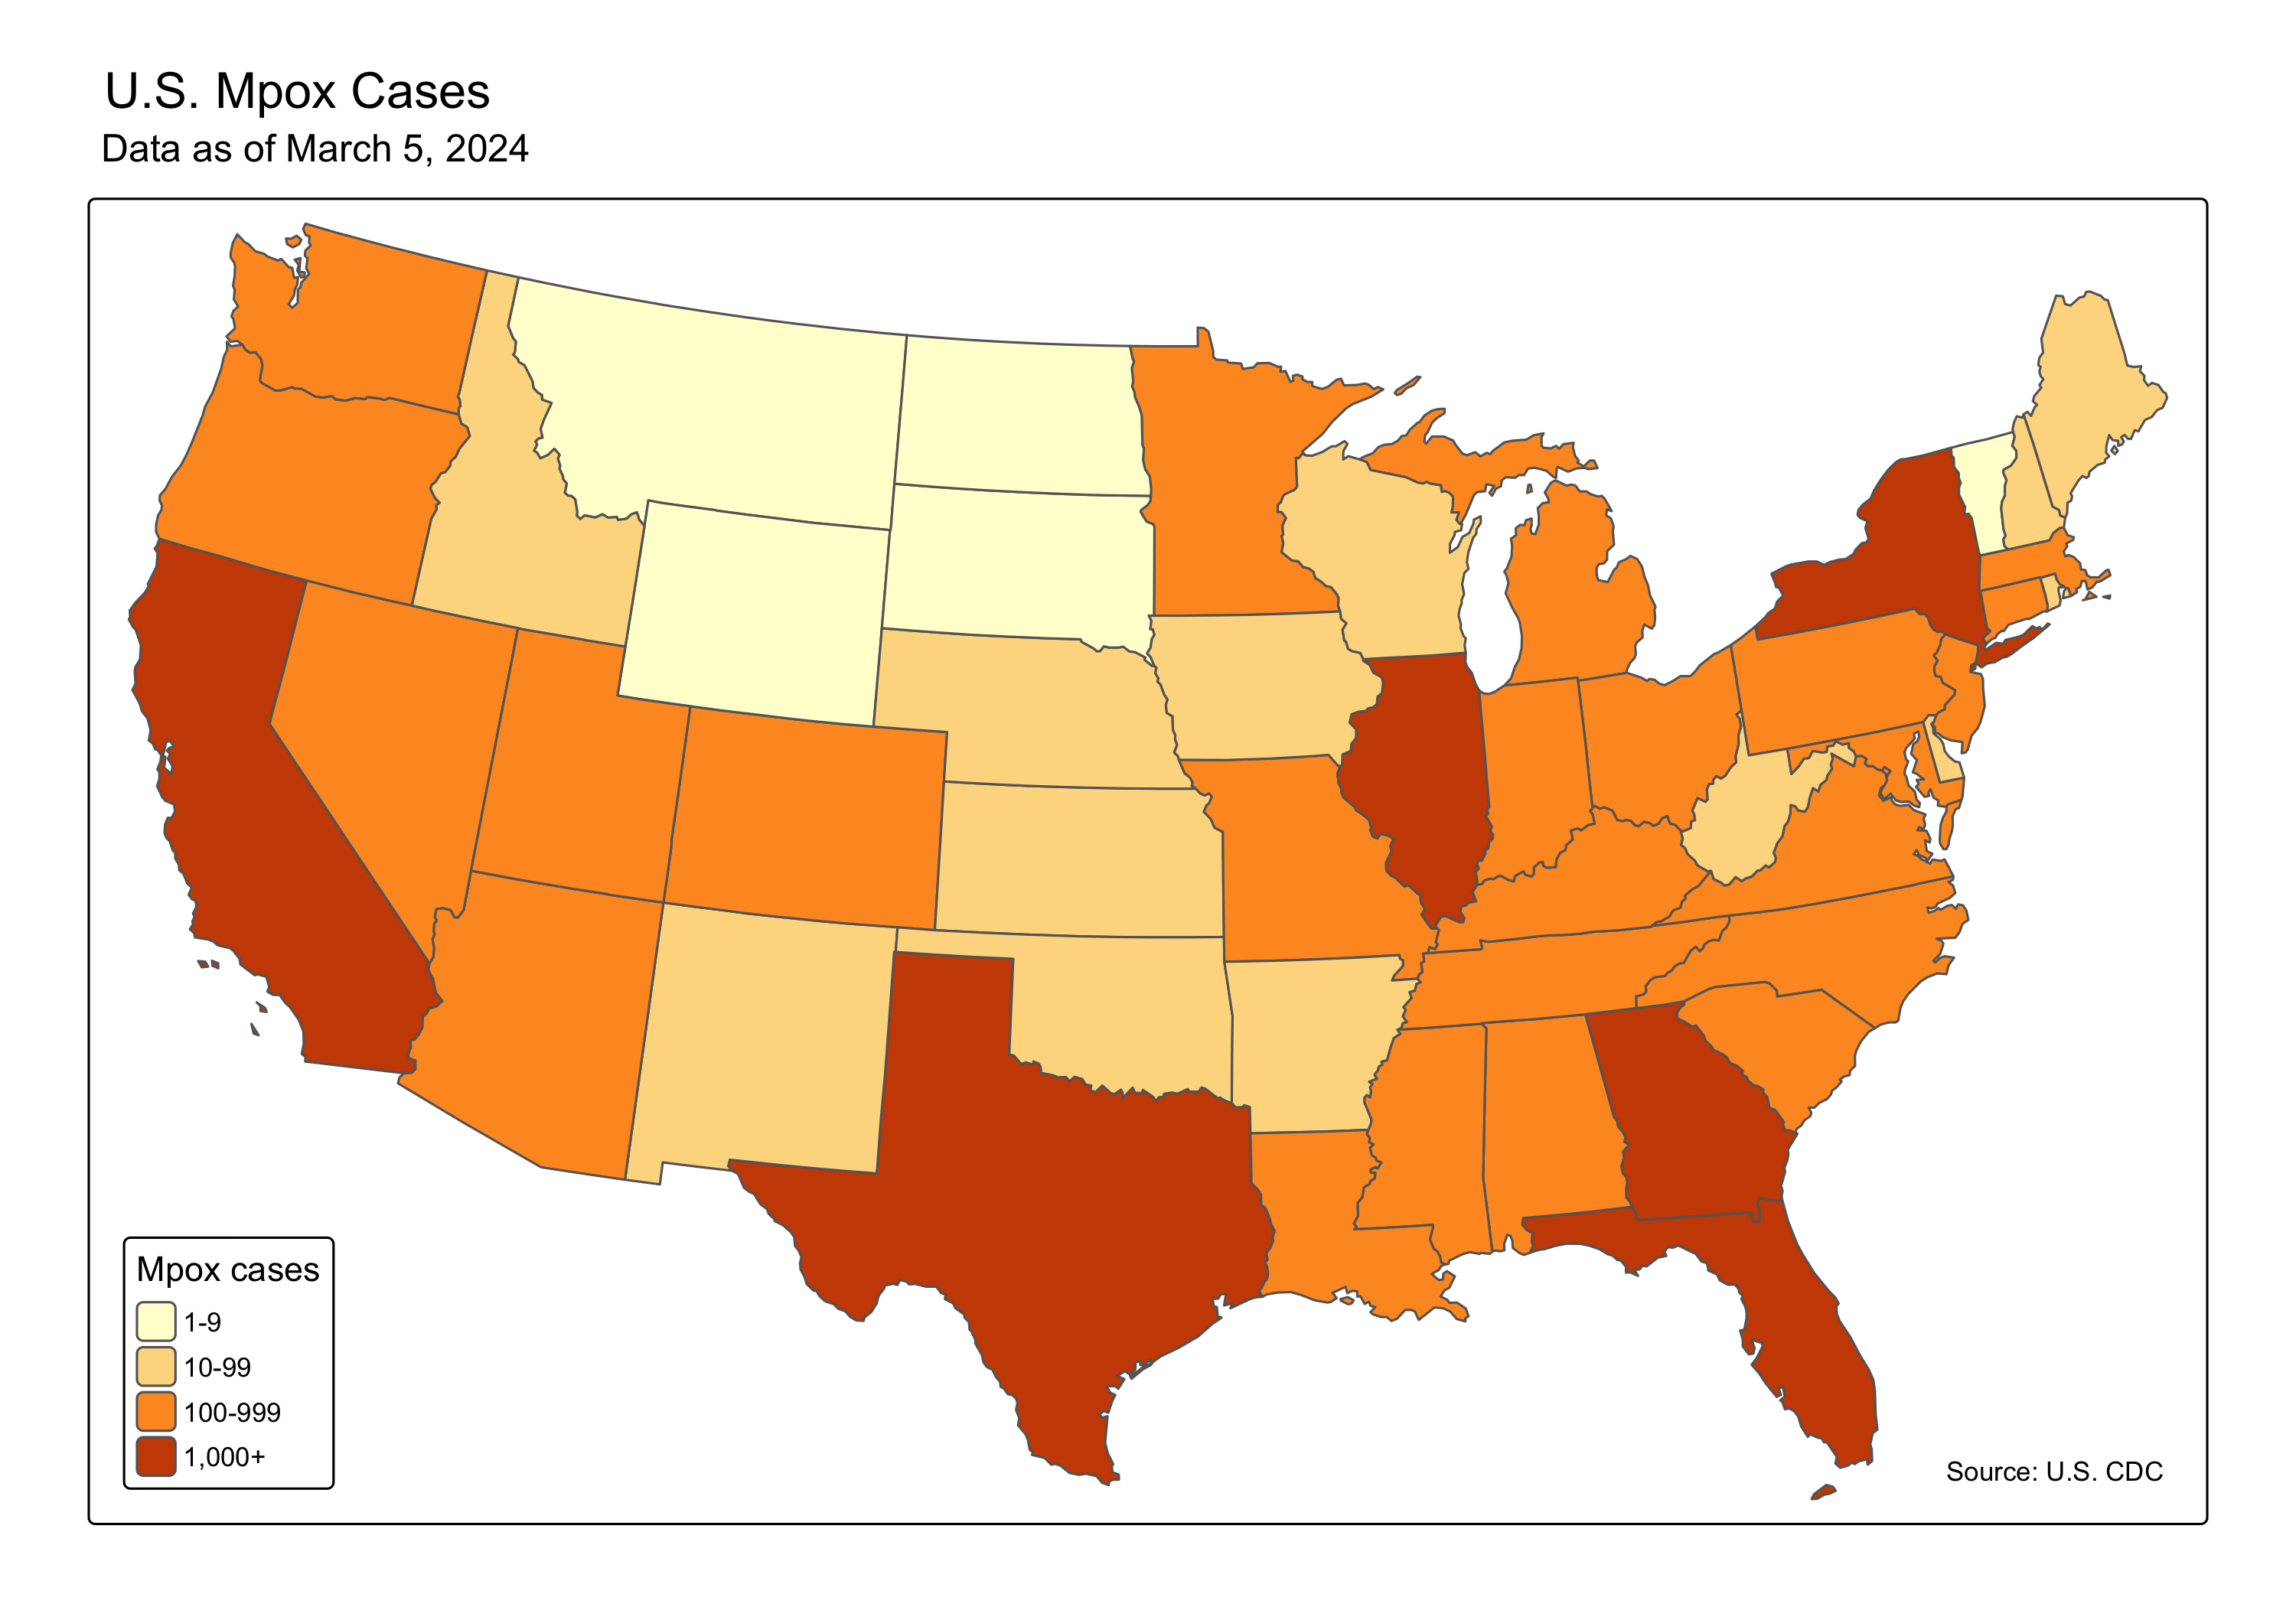
\includegraphics{images/mpox-cases-USA-states-map.png}

}

\caption{Note: Alaska (5 cases) and Hawaii (40 cases) are not depicted.}

\end{figure}%%
\begin{figure}[H]

{\centering 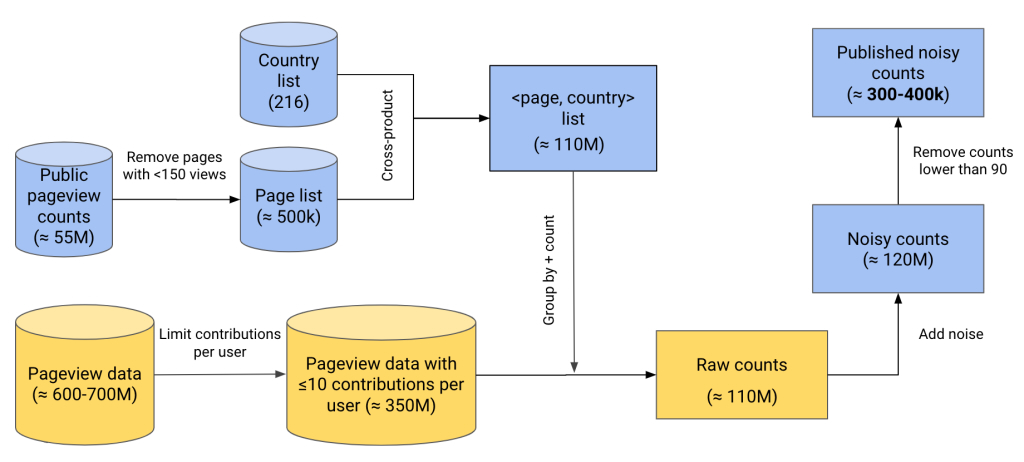
\includegraphics{images/wiki-pageview-differential-privacy-pipeline.jpg}

}

\caption{\href{https://diff.wikimedia.org/2023/06/21/new-dataset-uncovers-wikipedia-browsing-habits-while-protecting-users/screenshot-2023-05-23-at-10-34-18-am/}{Conceptual
Steps of the Pageview Differential Privacy Pipeline}, a
\href{https://creativecommons.org/licenses/by-sa/4.0/}{CC BY-SA 4.0}
licensed work by Hal Triedman}

\end{figure}%

\begin{center}
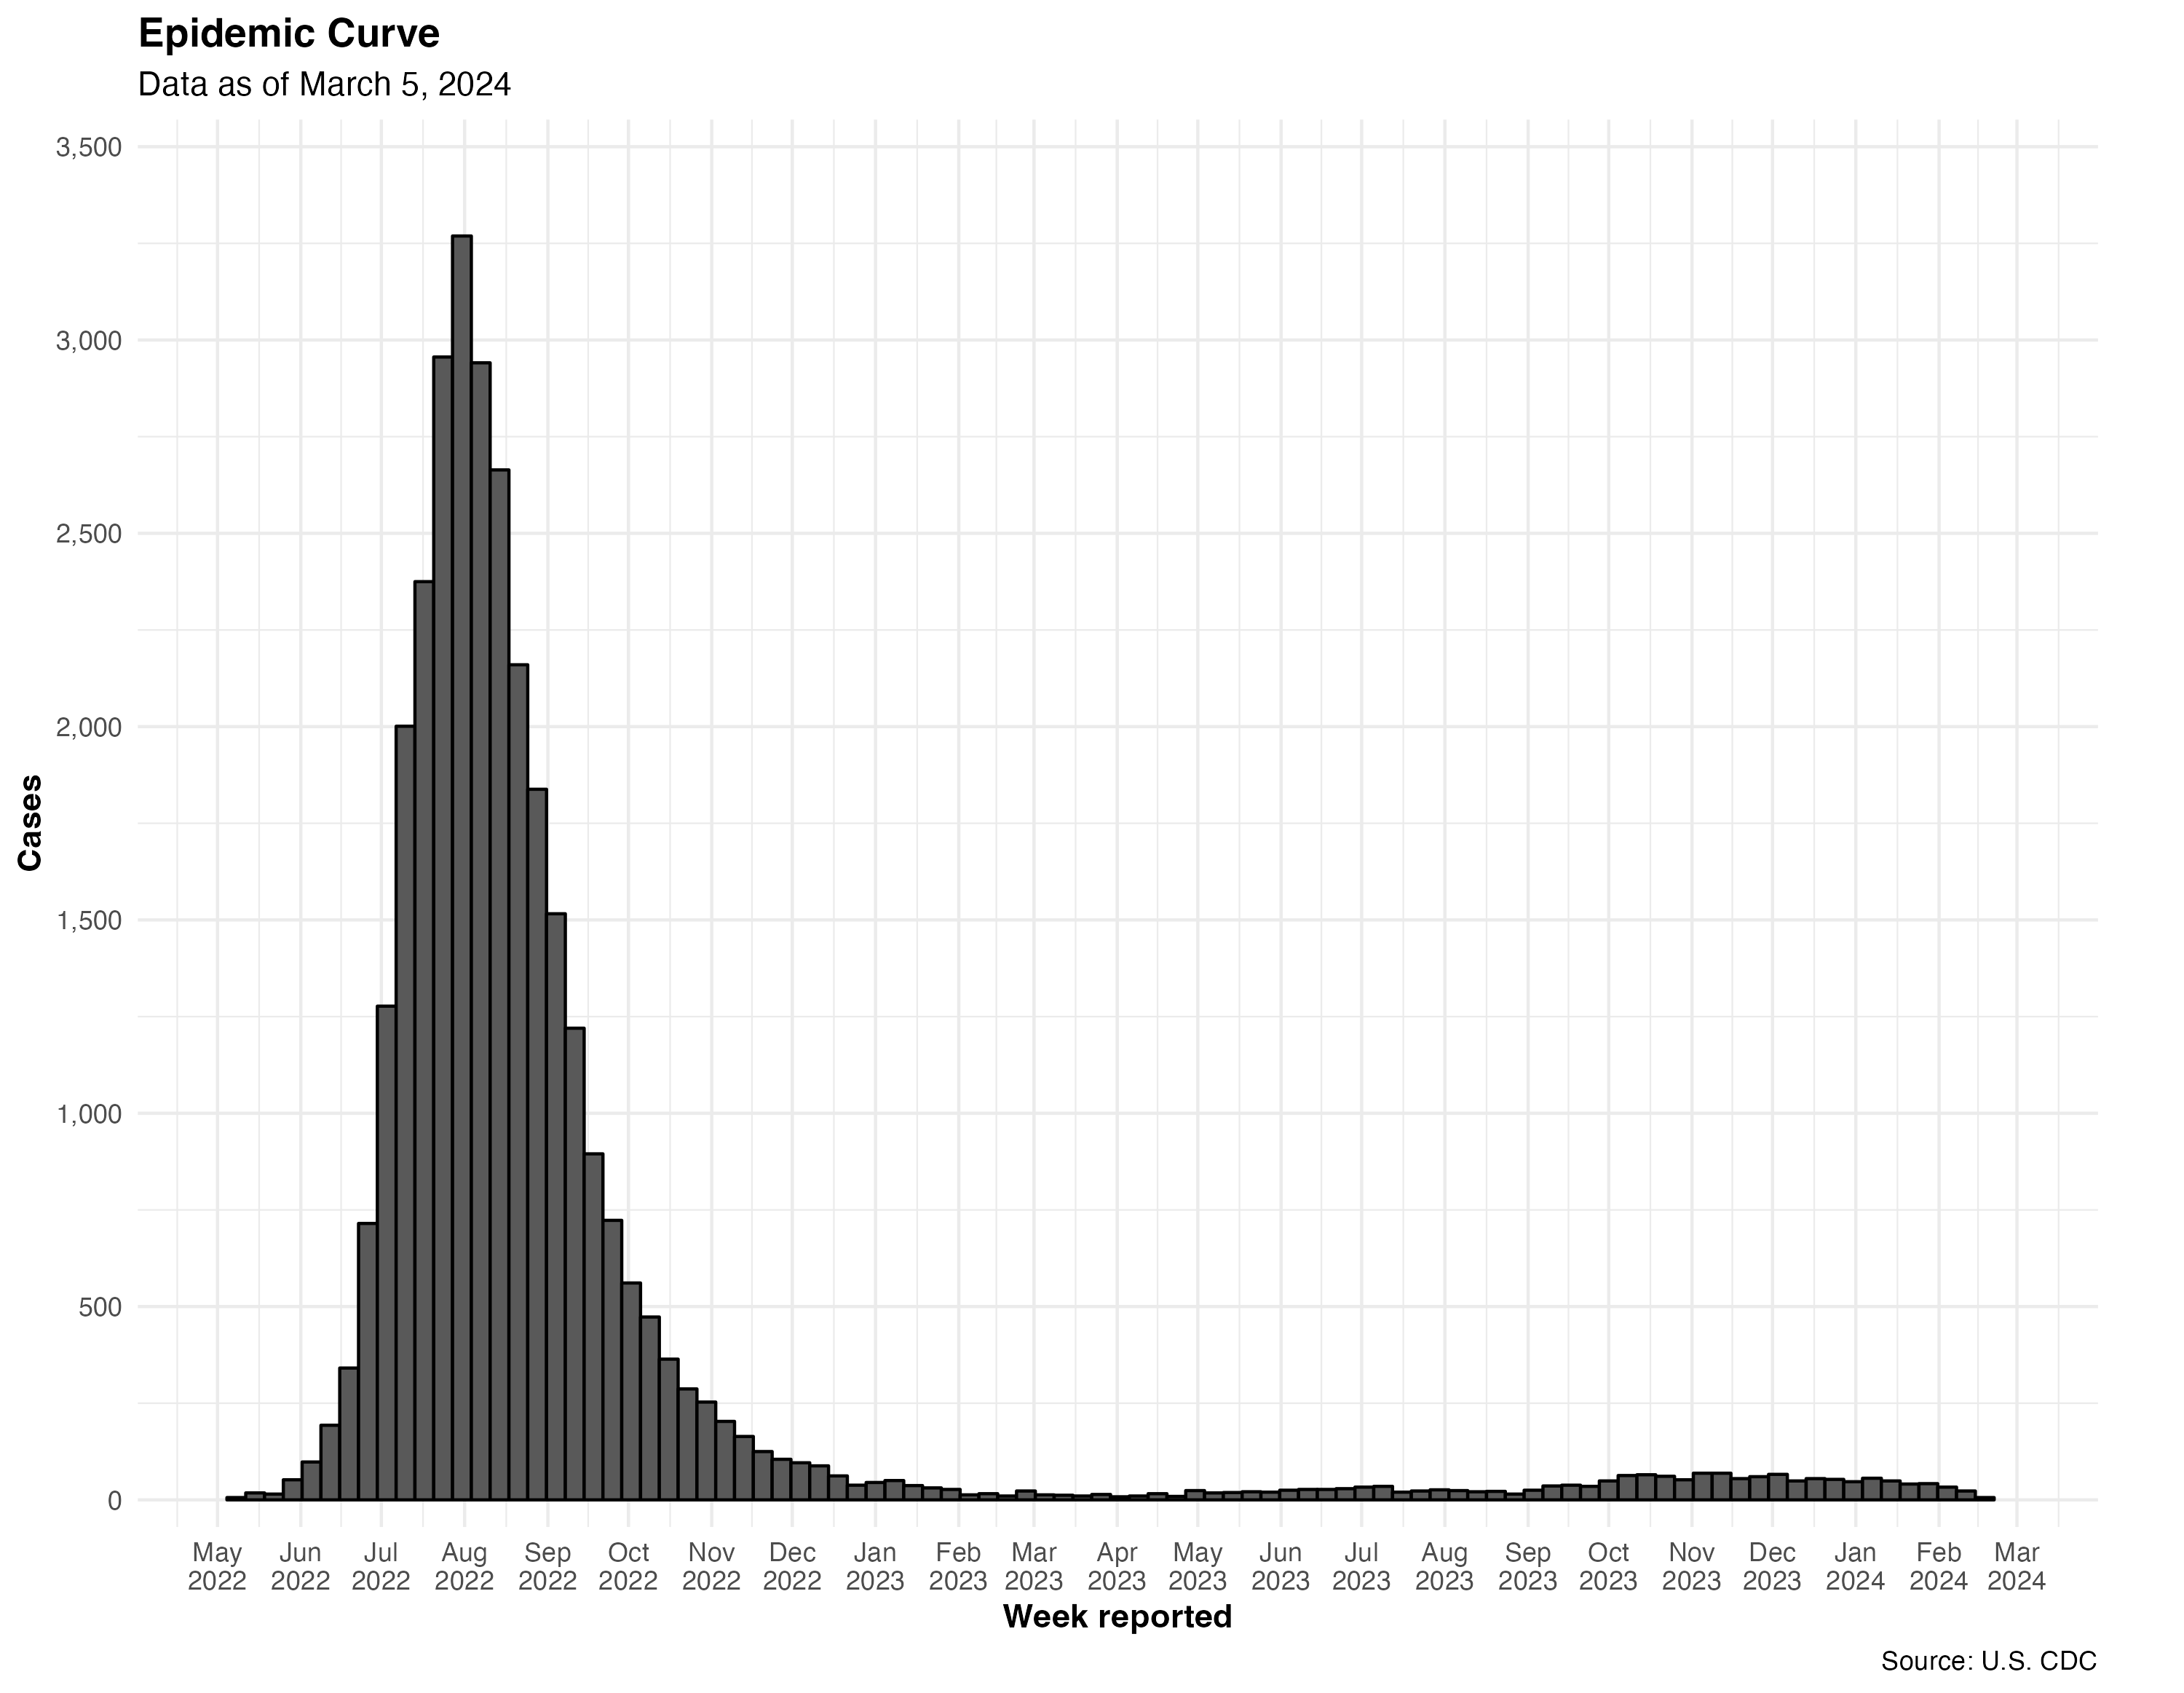
\includegraphics{images/mpox-cases-USA-weekly.png}
\end{center}

\begin{center}
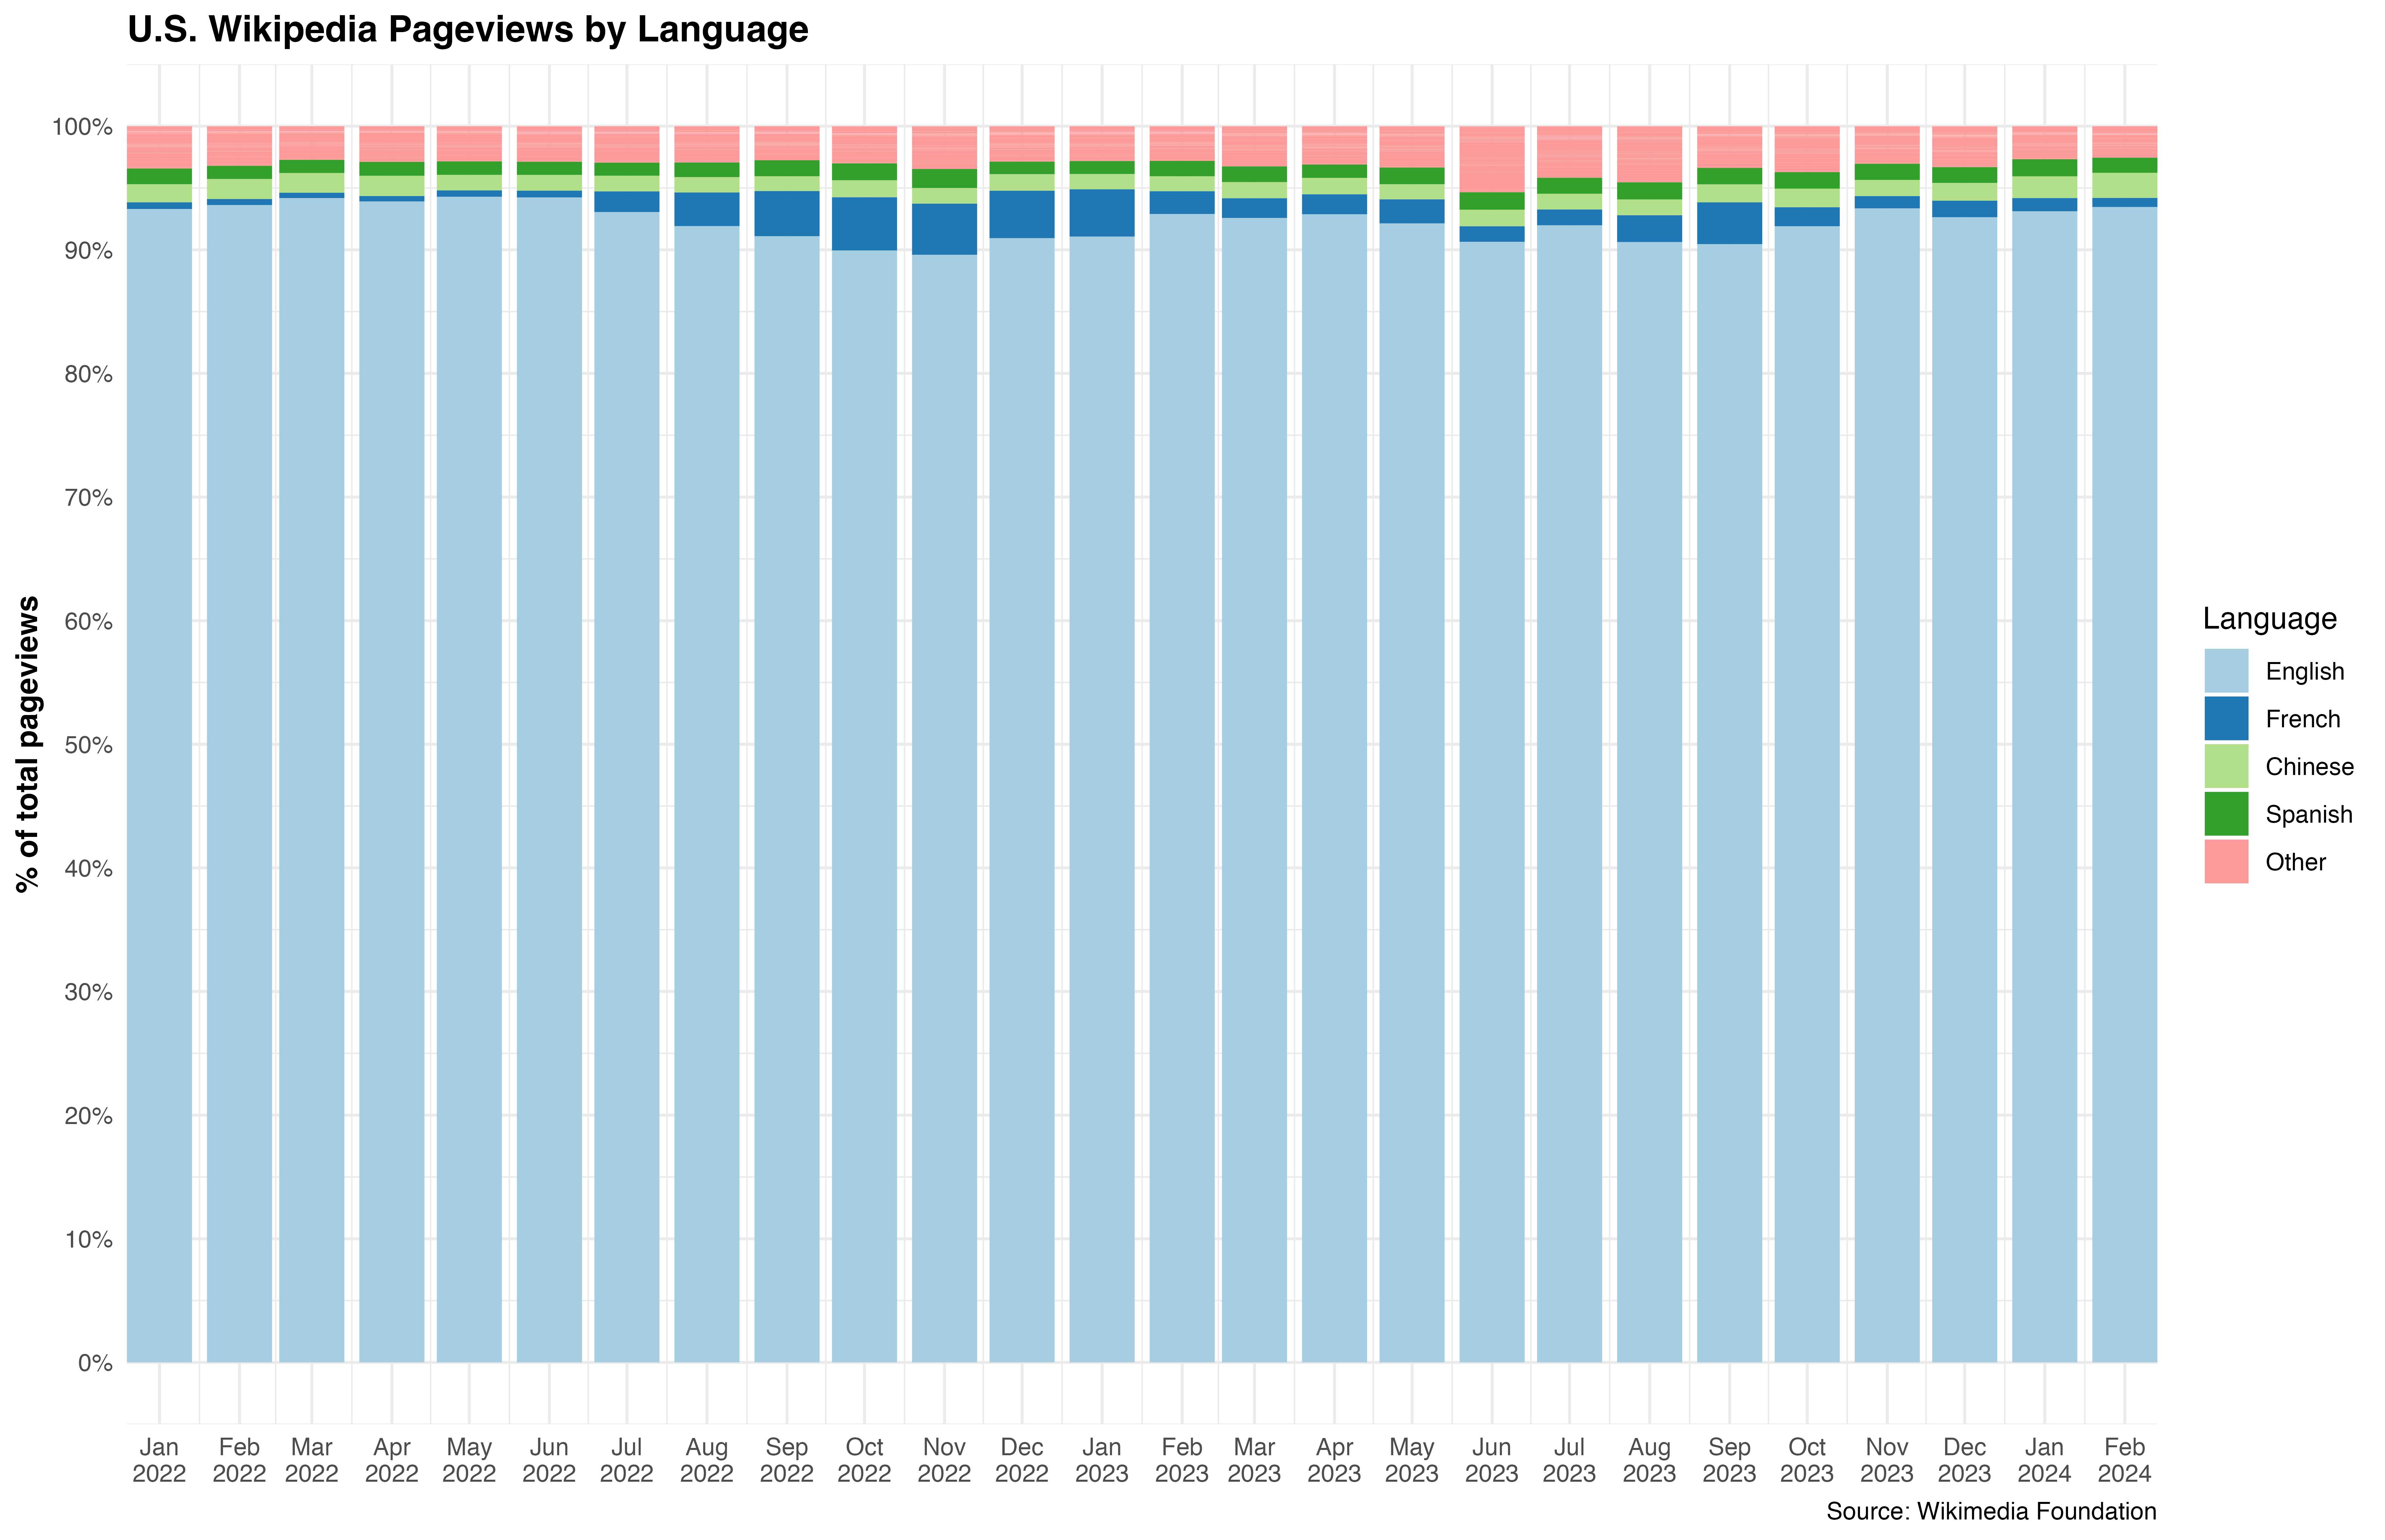
\includegraphics{images/wiki-project-views-USA-monthly.png}
\end{center}

\begin{center}
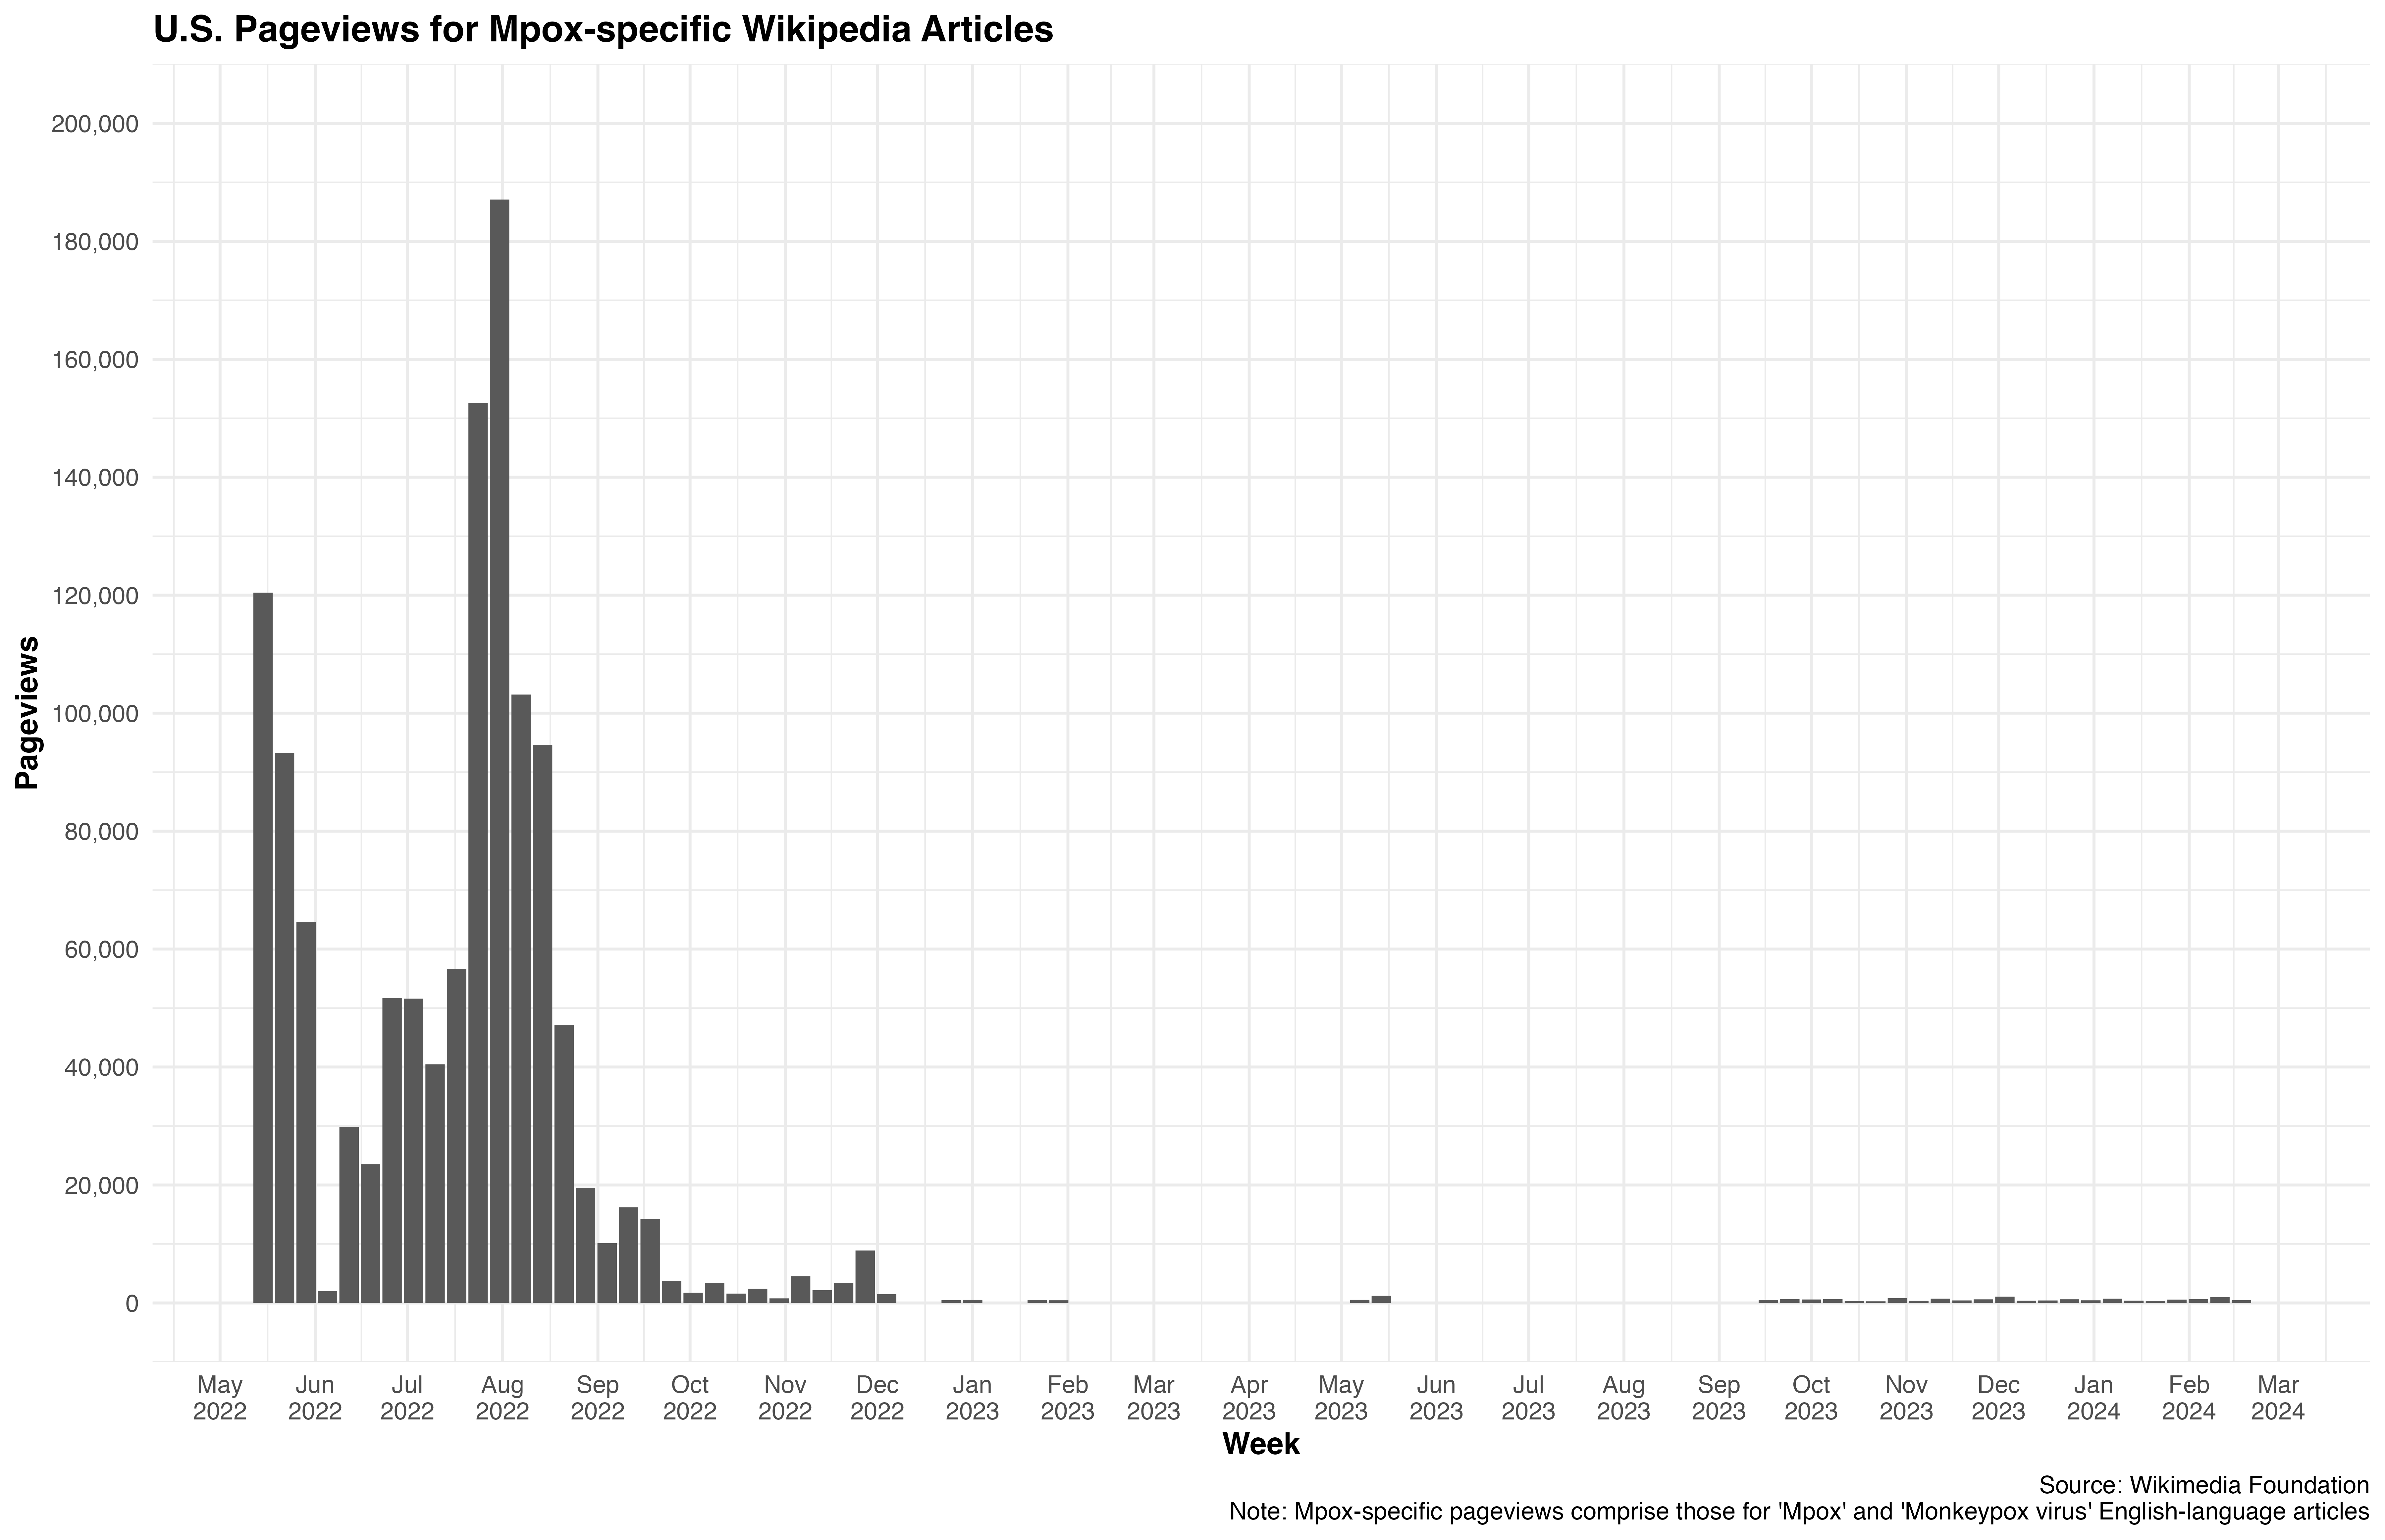
\includegraphics{images/wiki-pageviews-mpox-specific-USA-weekly-01.png}
\end{center}

\begin{center}
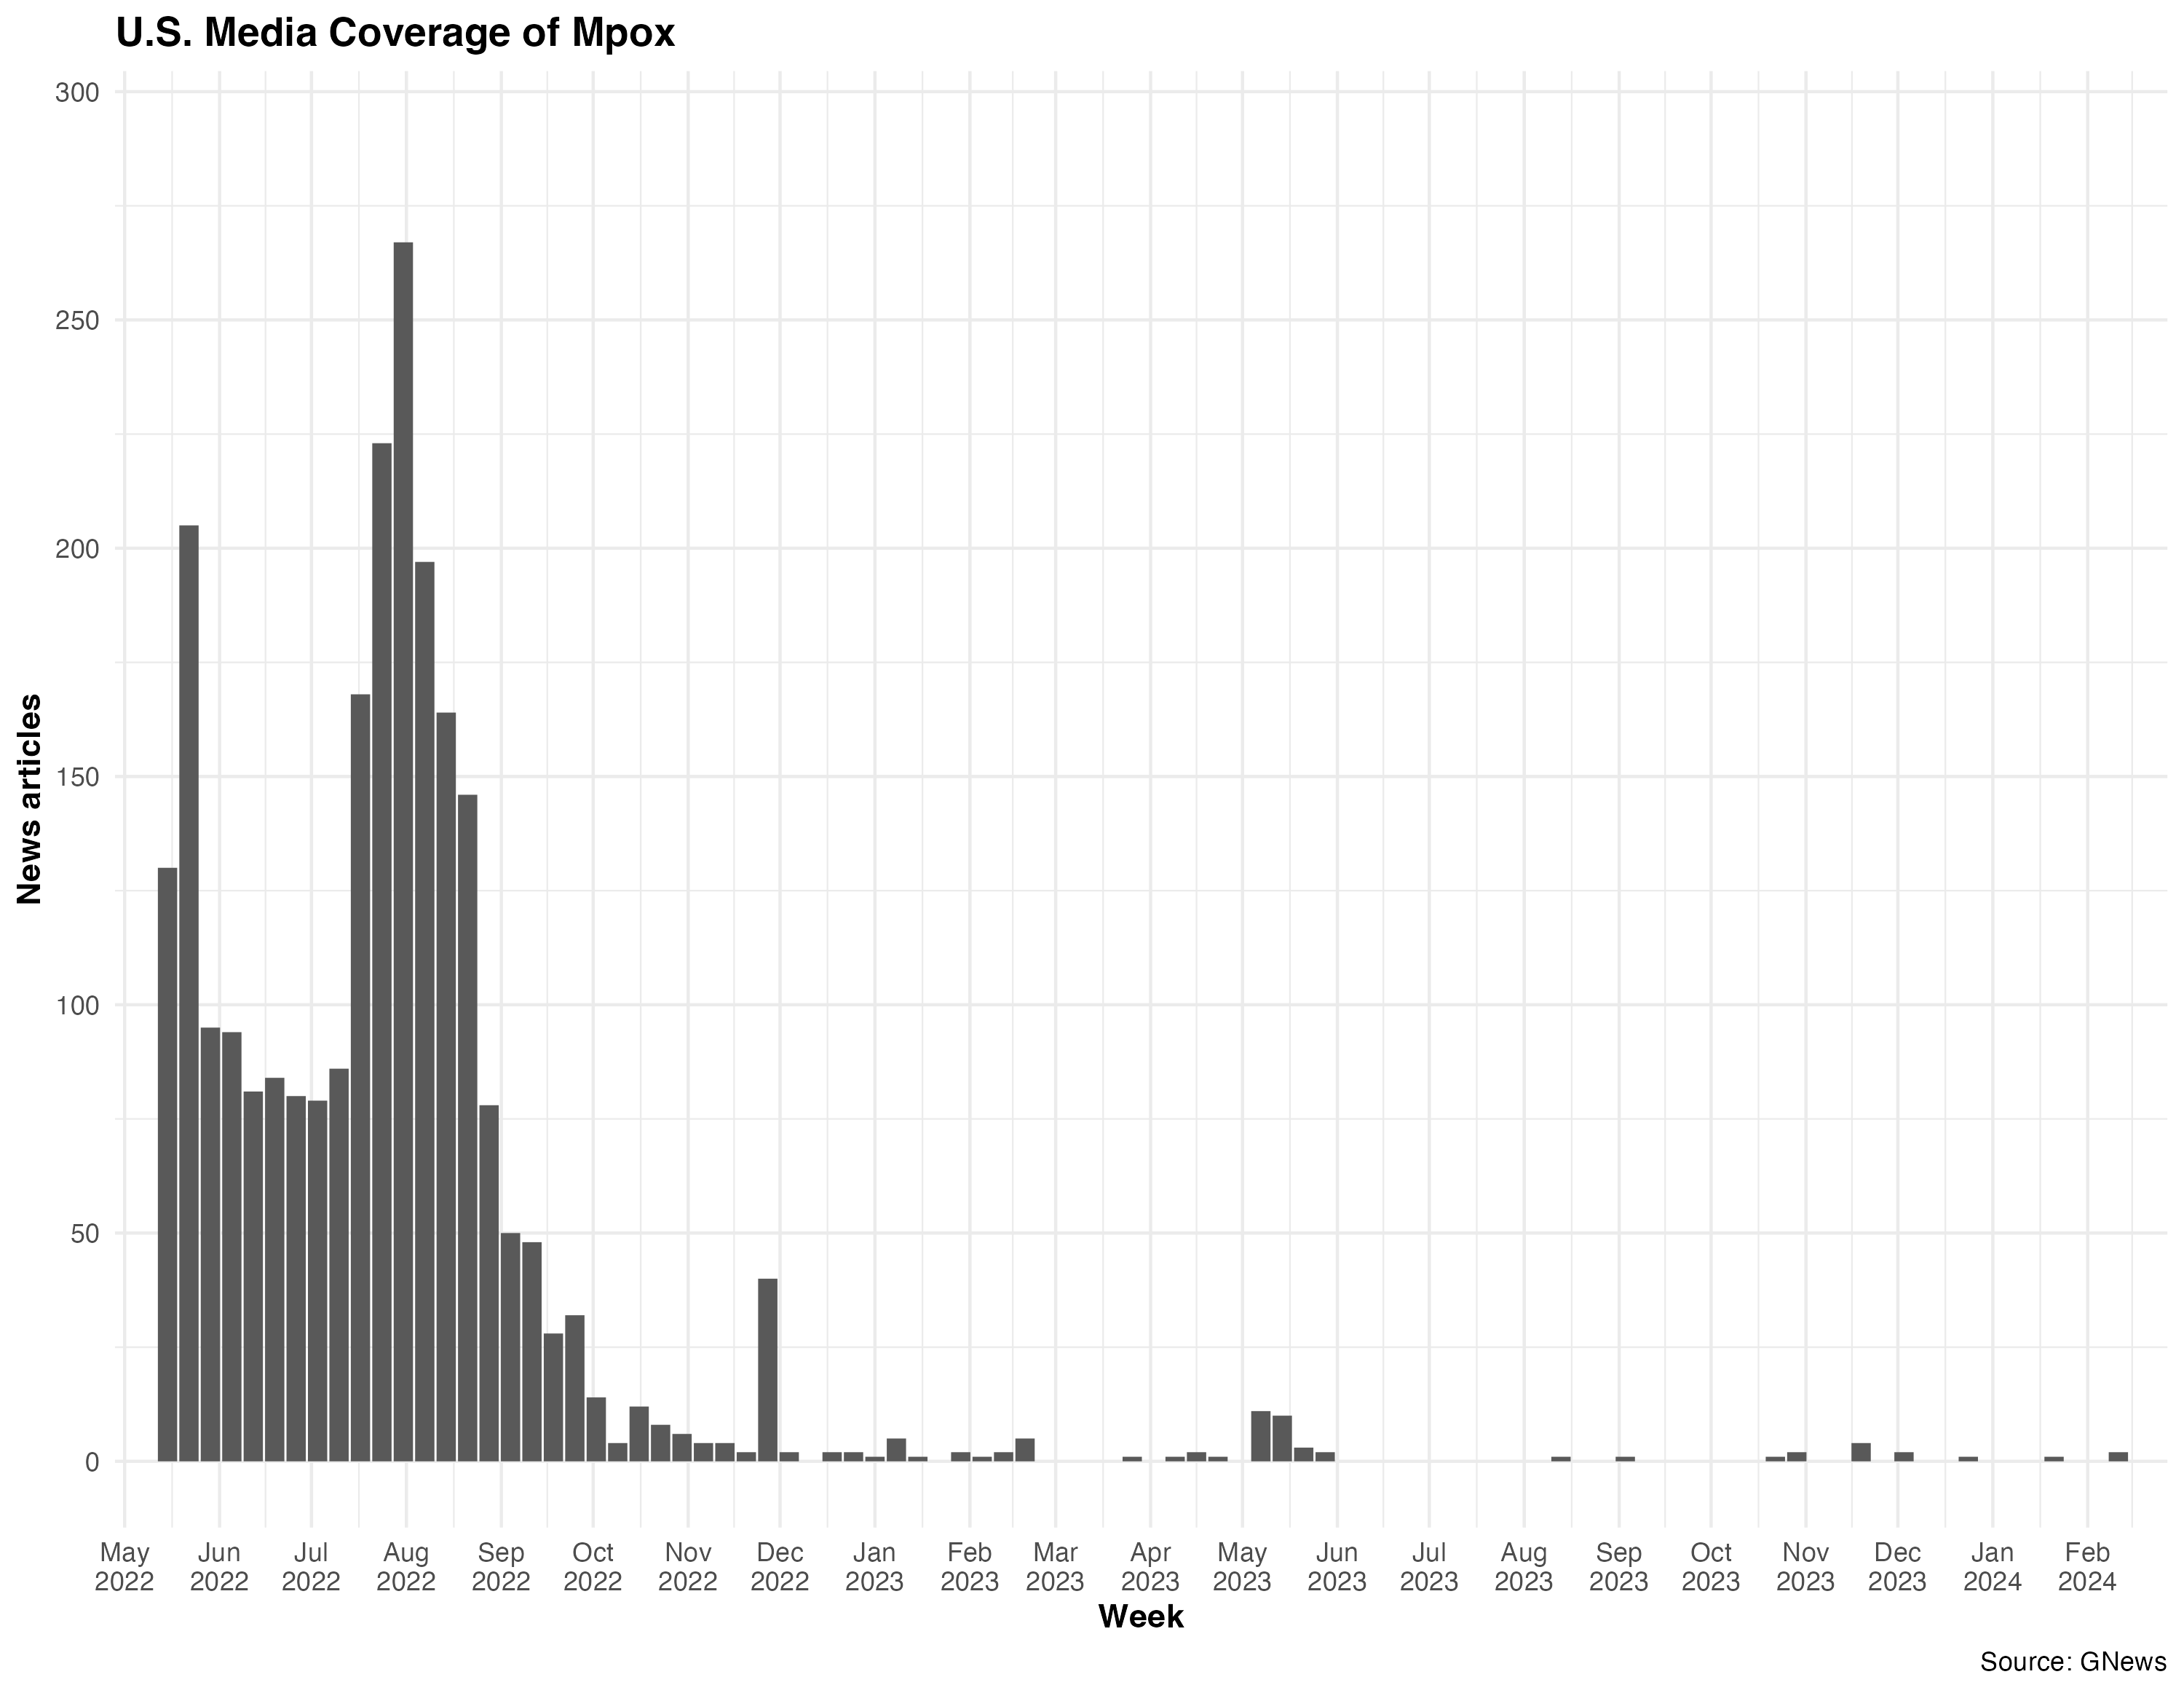
\includegraphics{images/mpox-news-USA-weekly.png}
\end{center}

\begin{center}
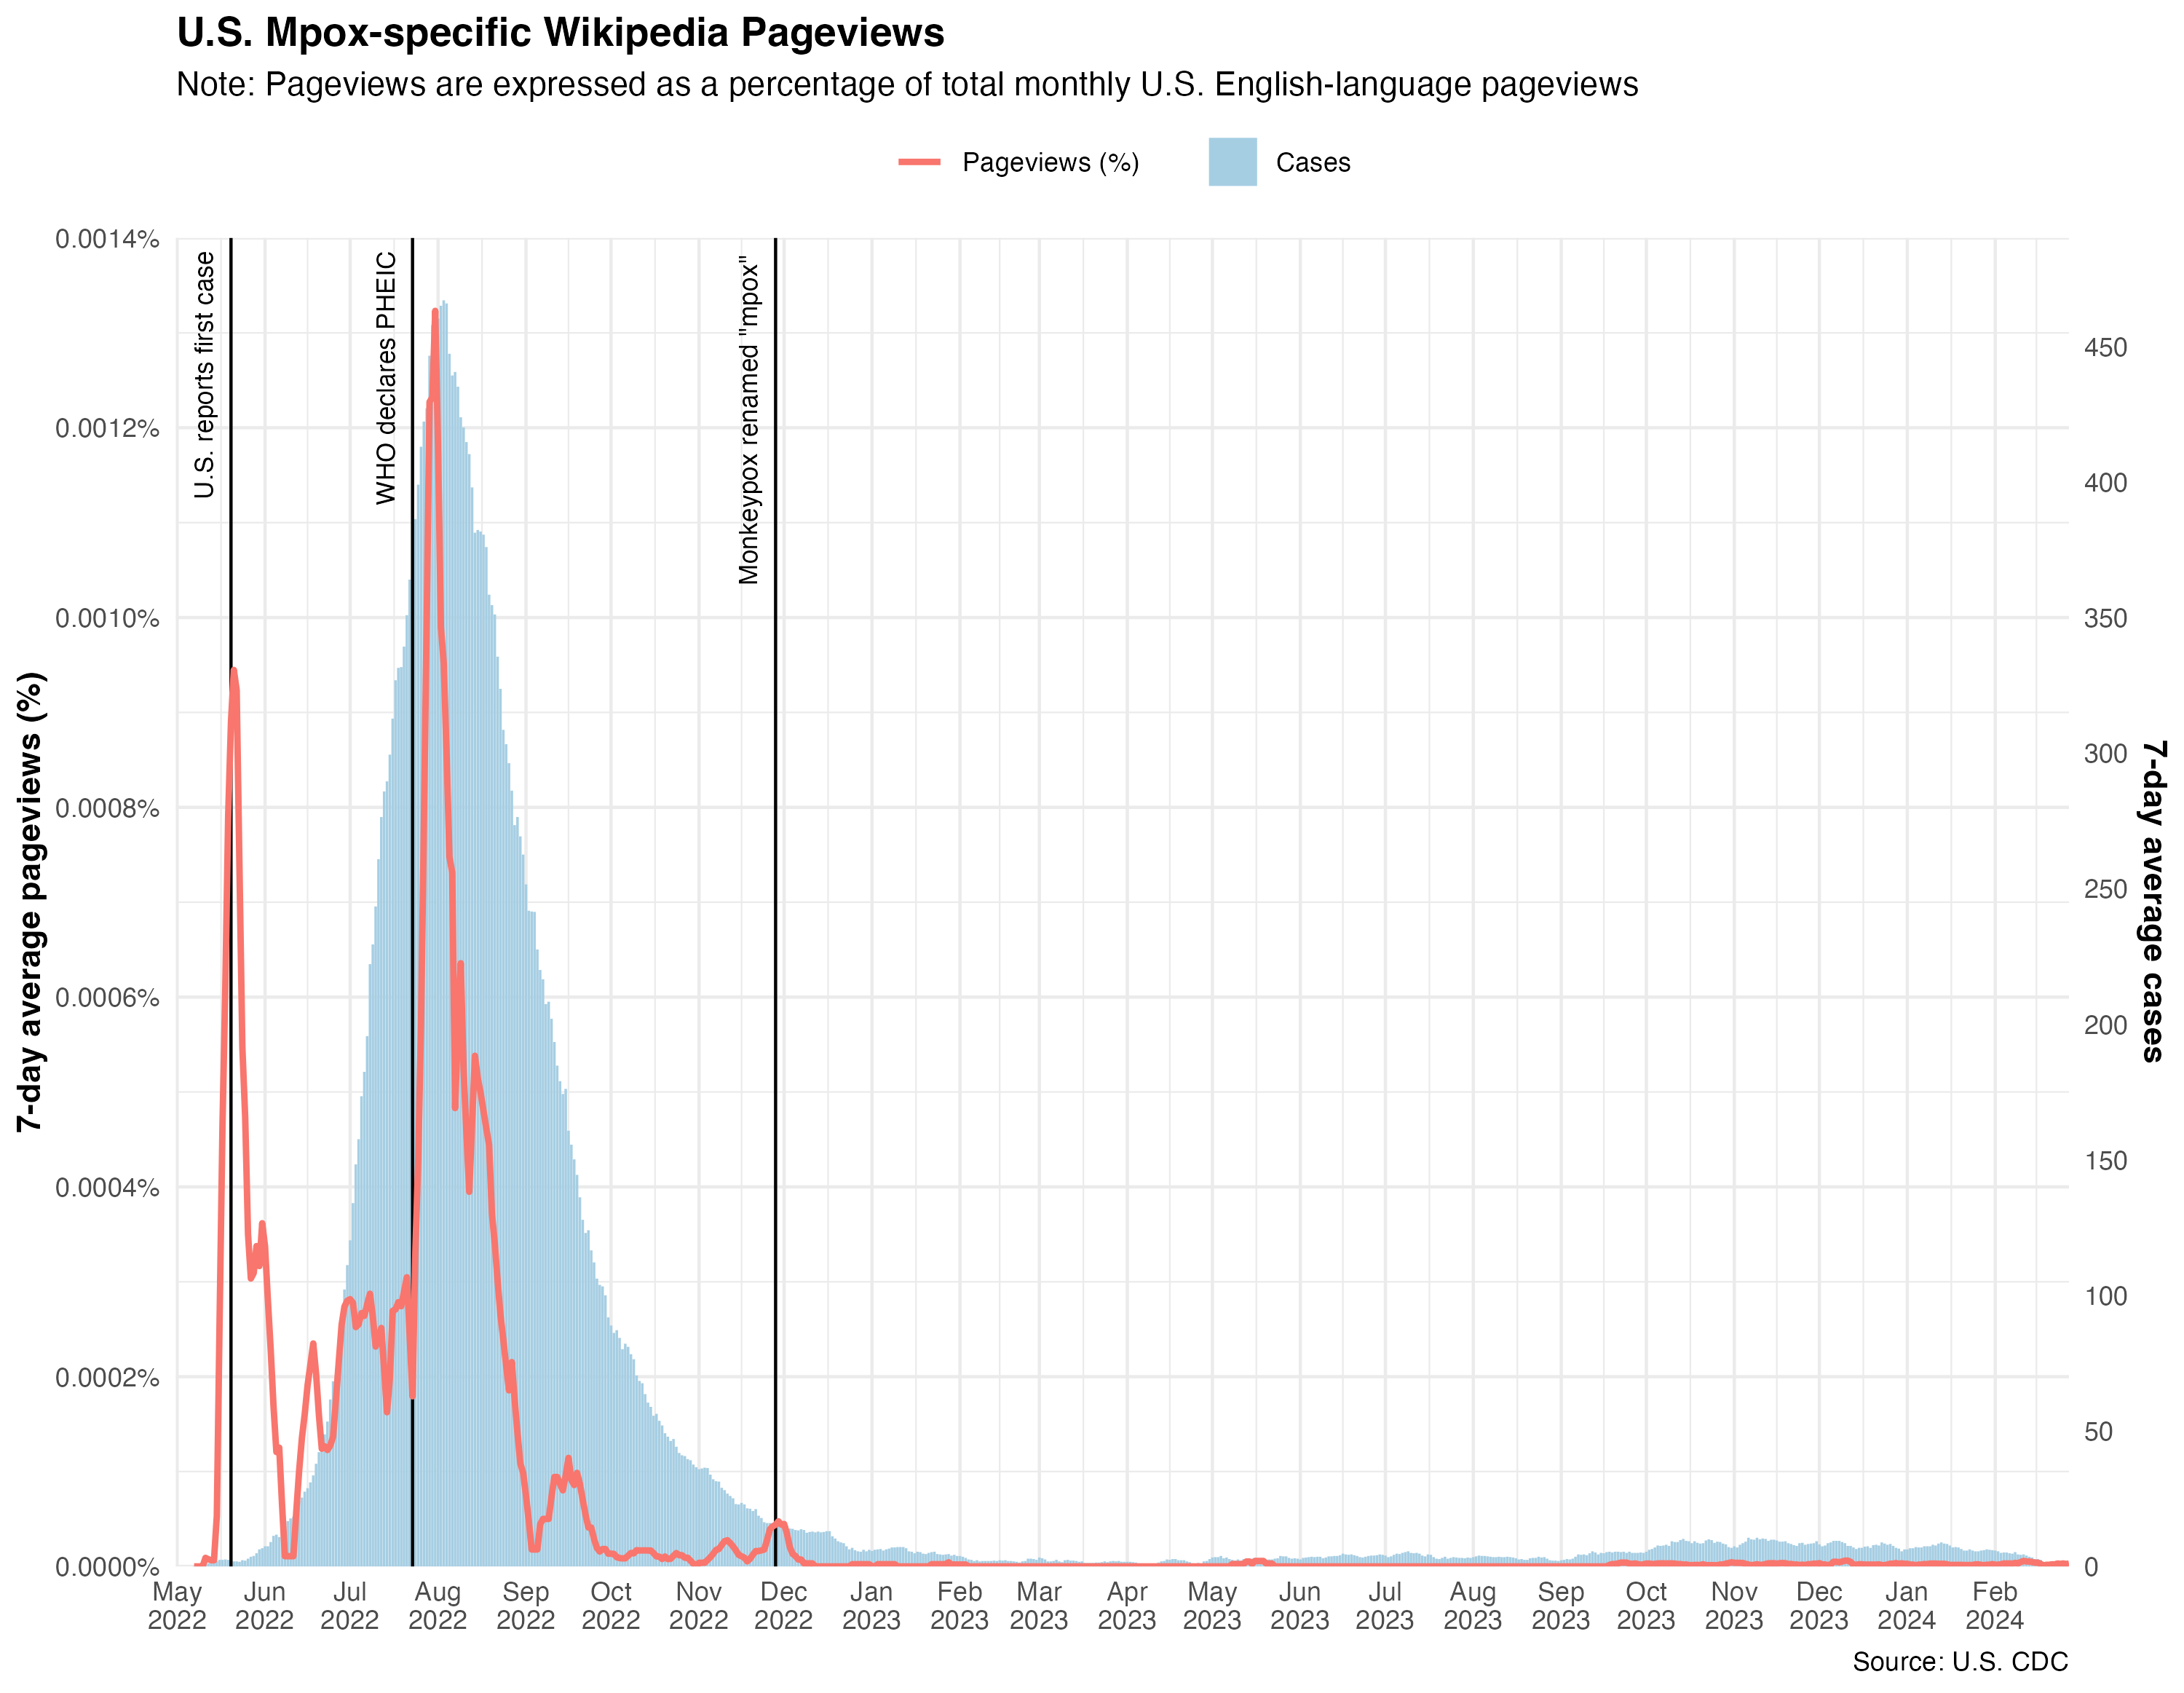
\includegraphics{images/mpox-cases-&-wiki-pageviews-USA-rolling-avg.png}
\end{center}

\begin{center}
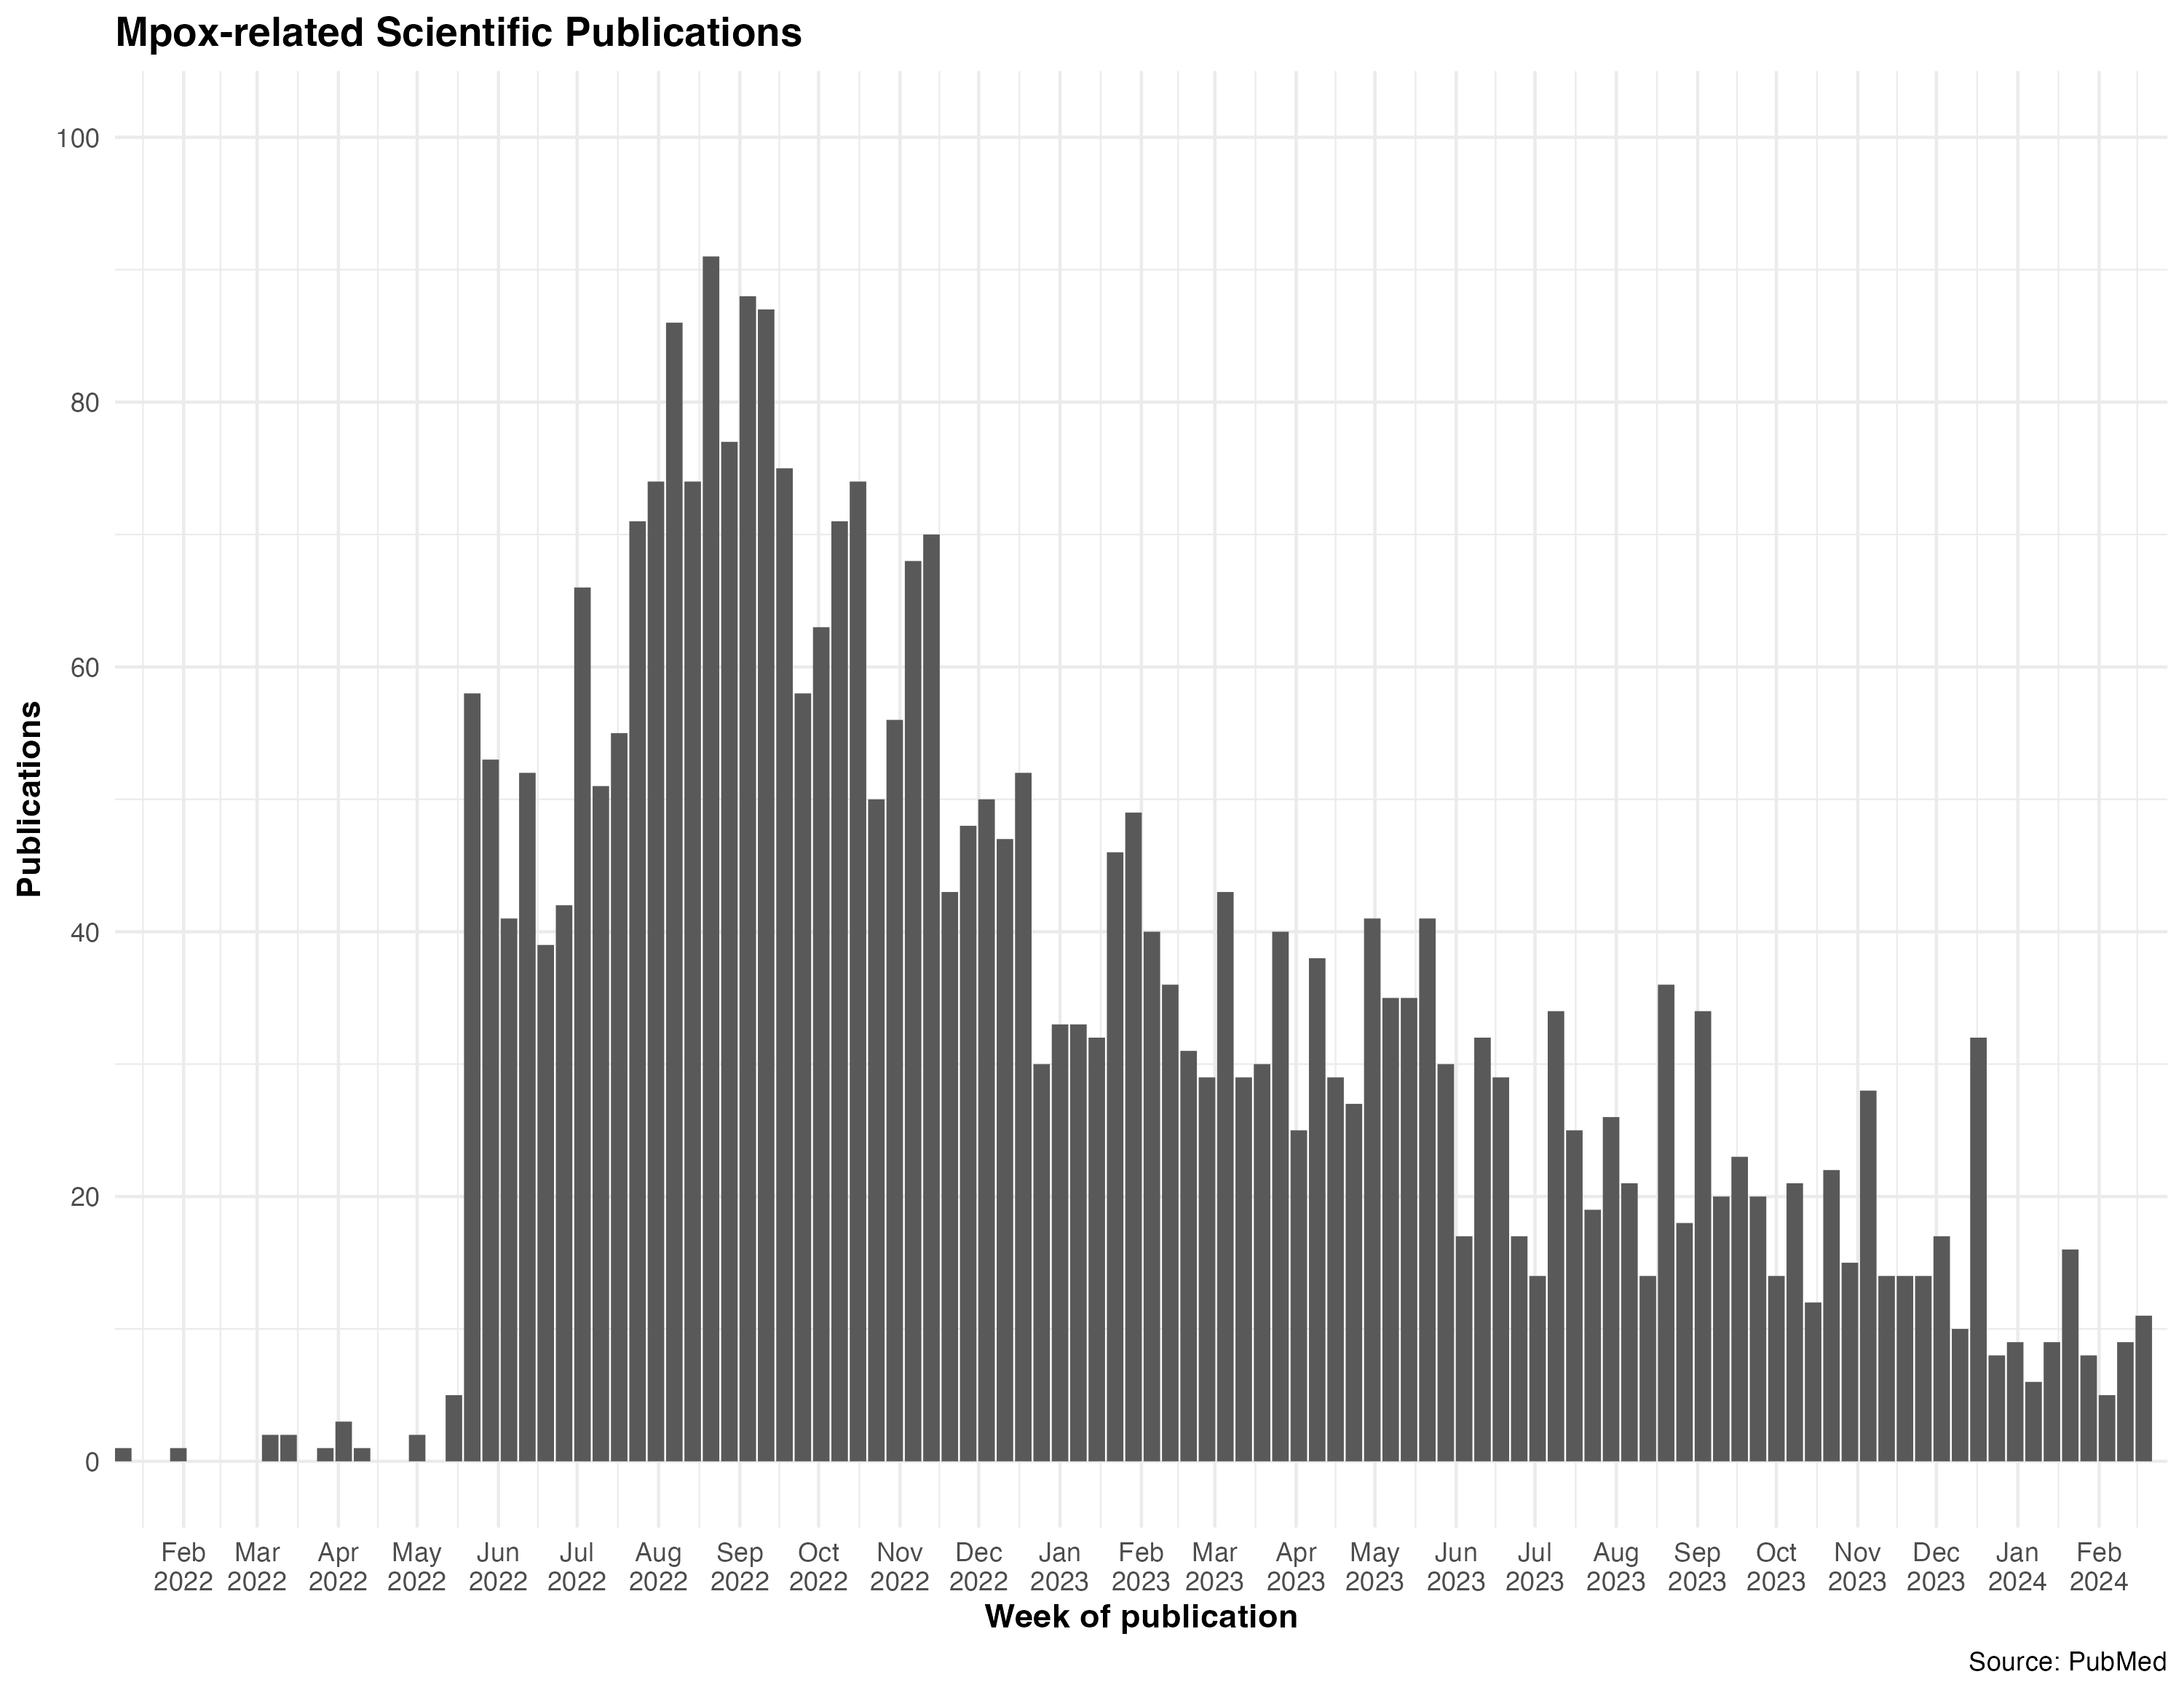
\includegraphics{images/mpox-studies-USA-weekly.png}
\end{center}

\begin{center}
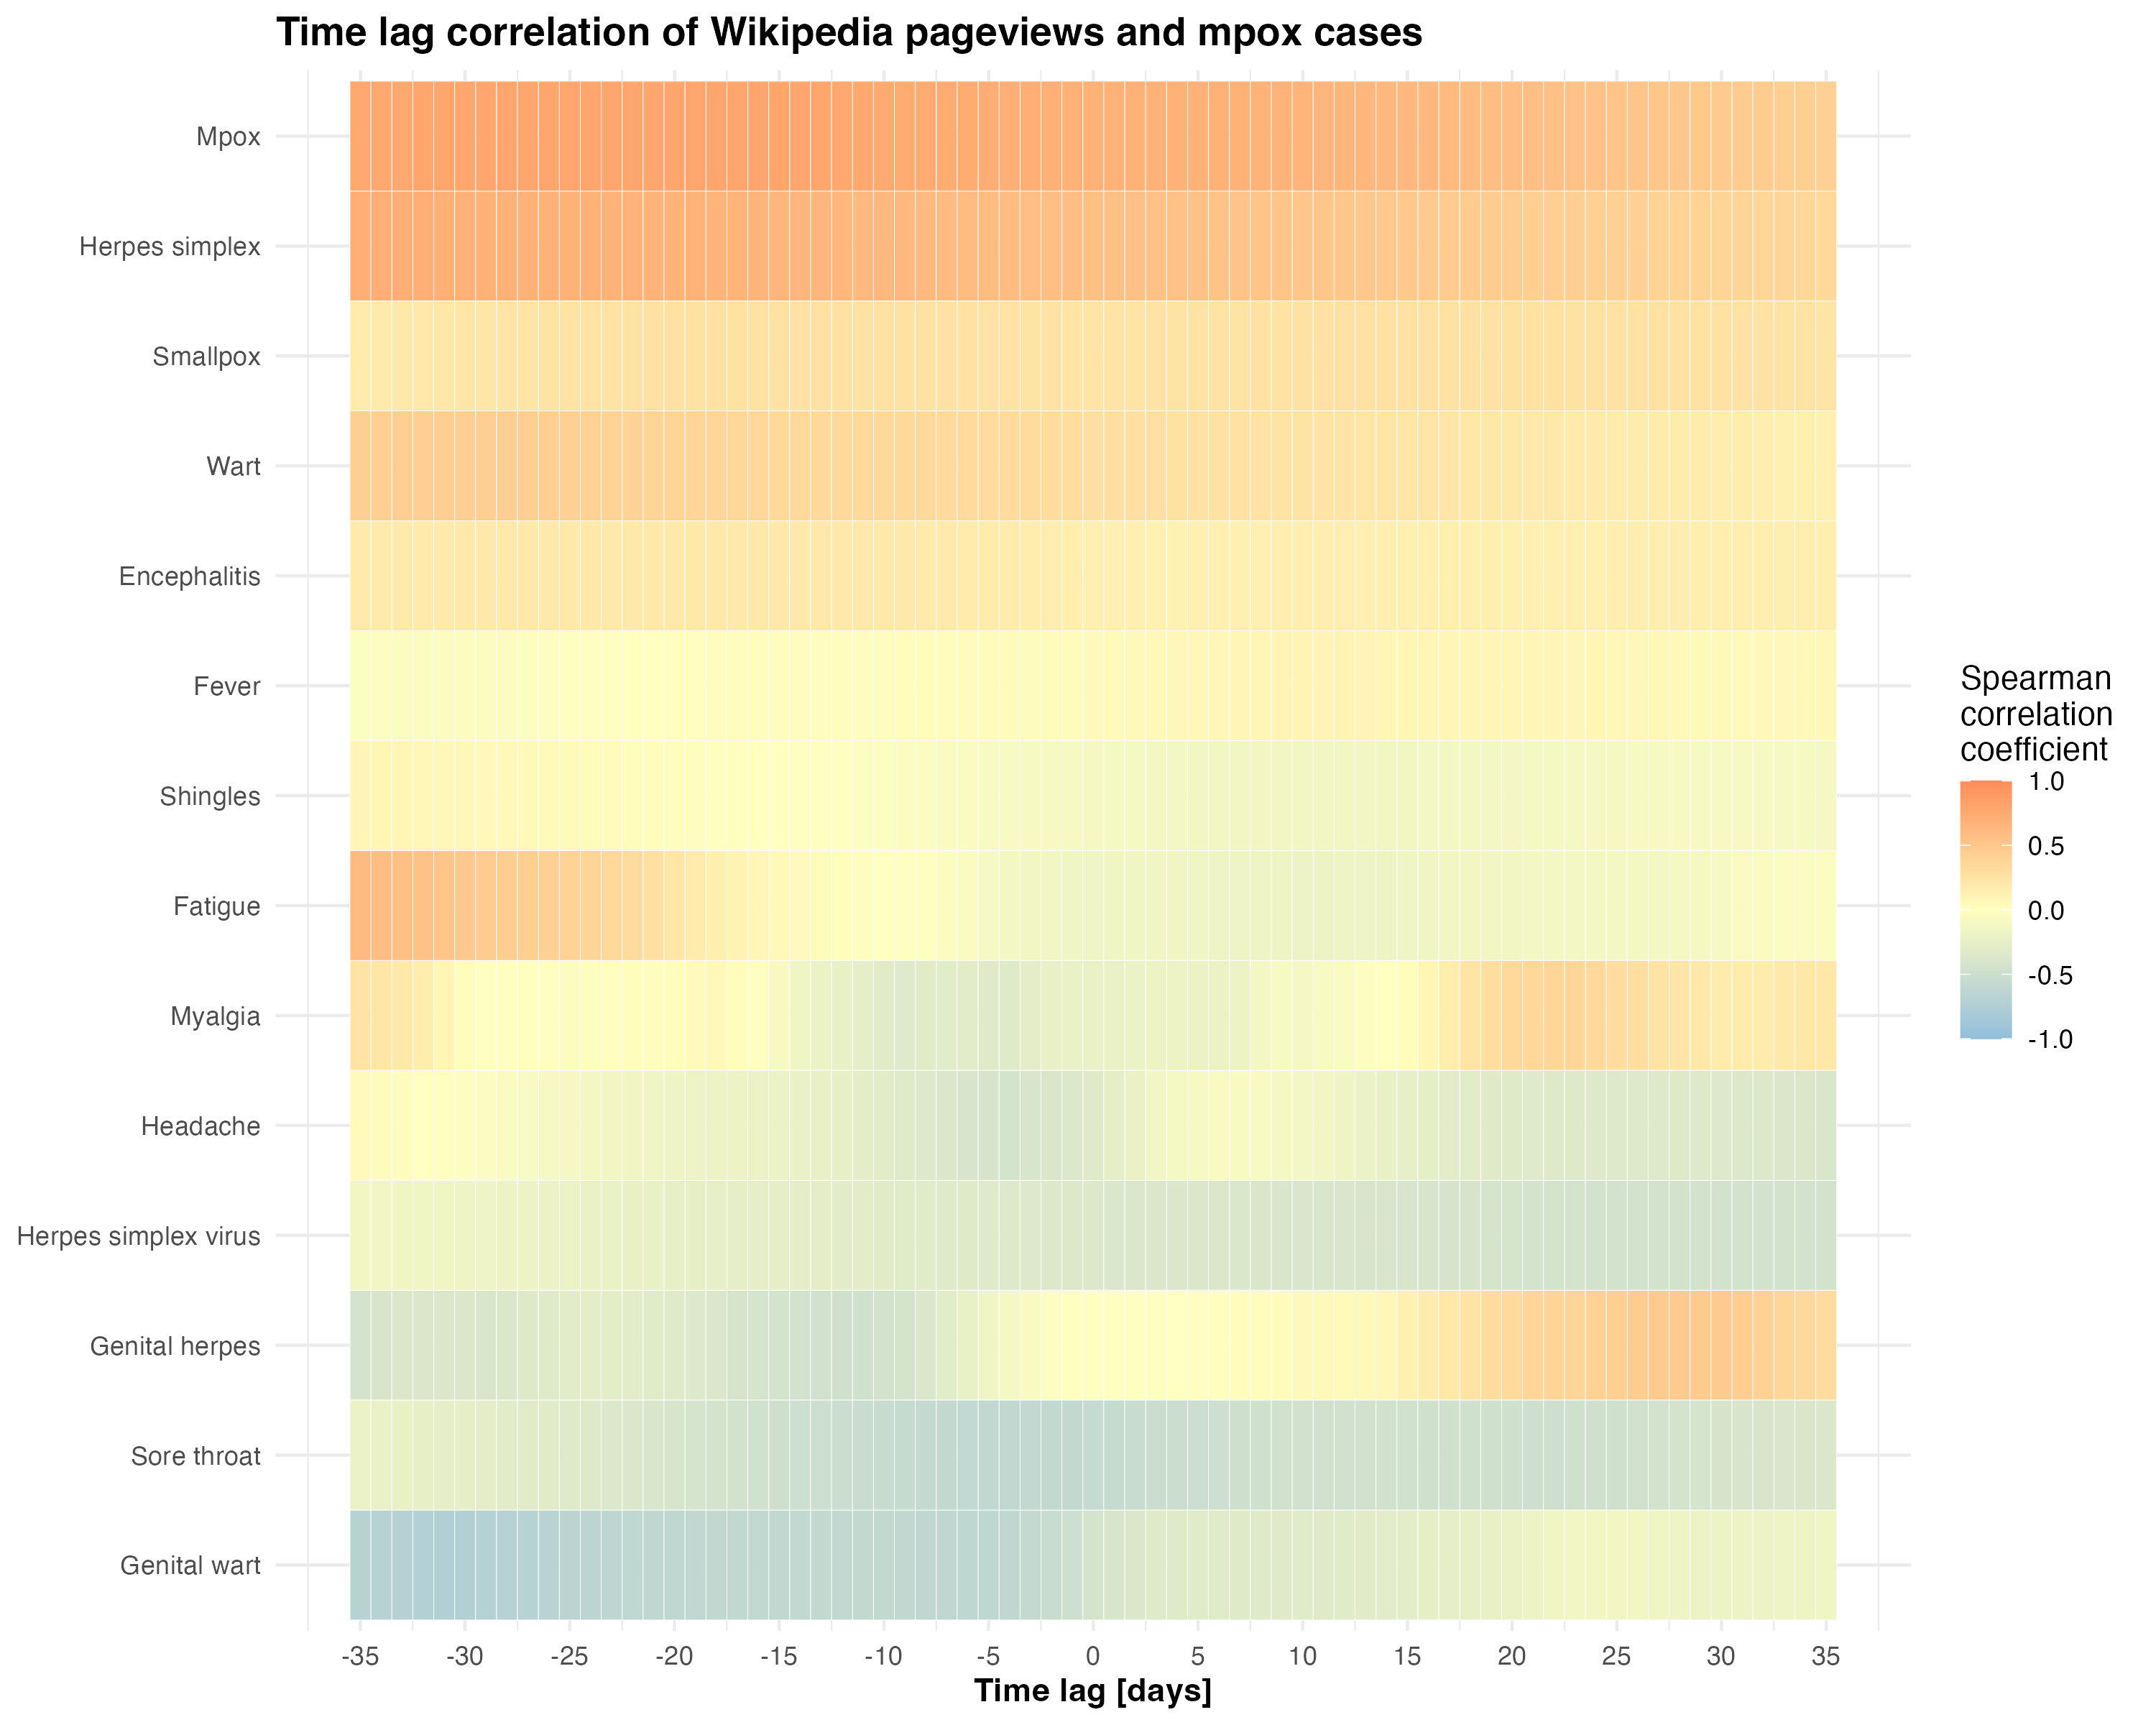
\includegraphics{images/spearman-correlation-heatmap.png}
\end{center}

\begin{center}
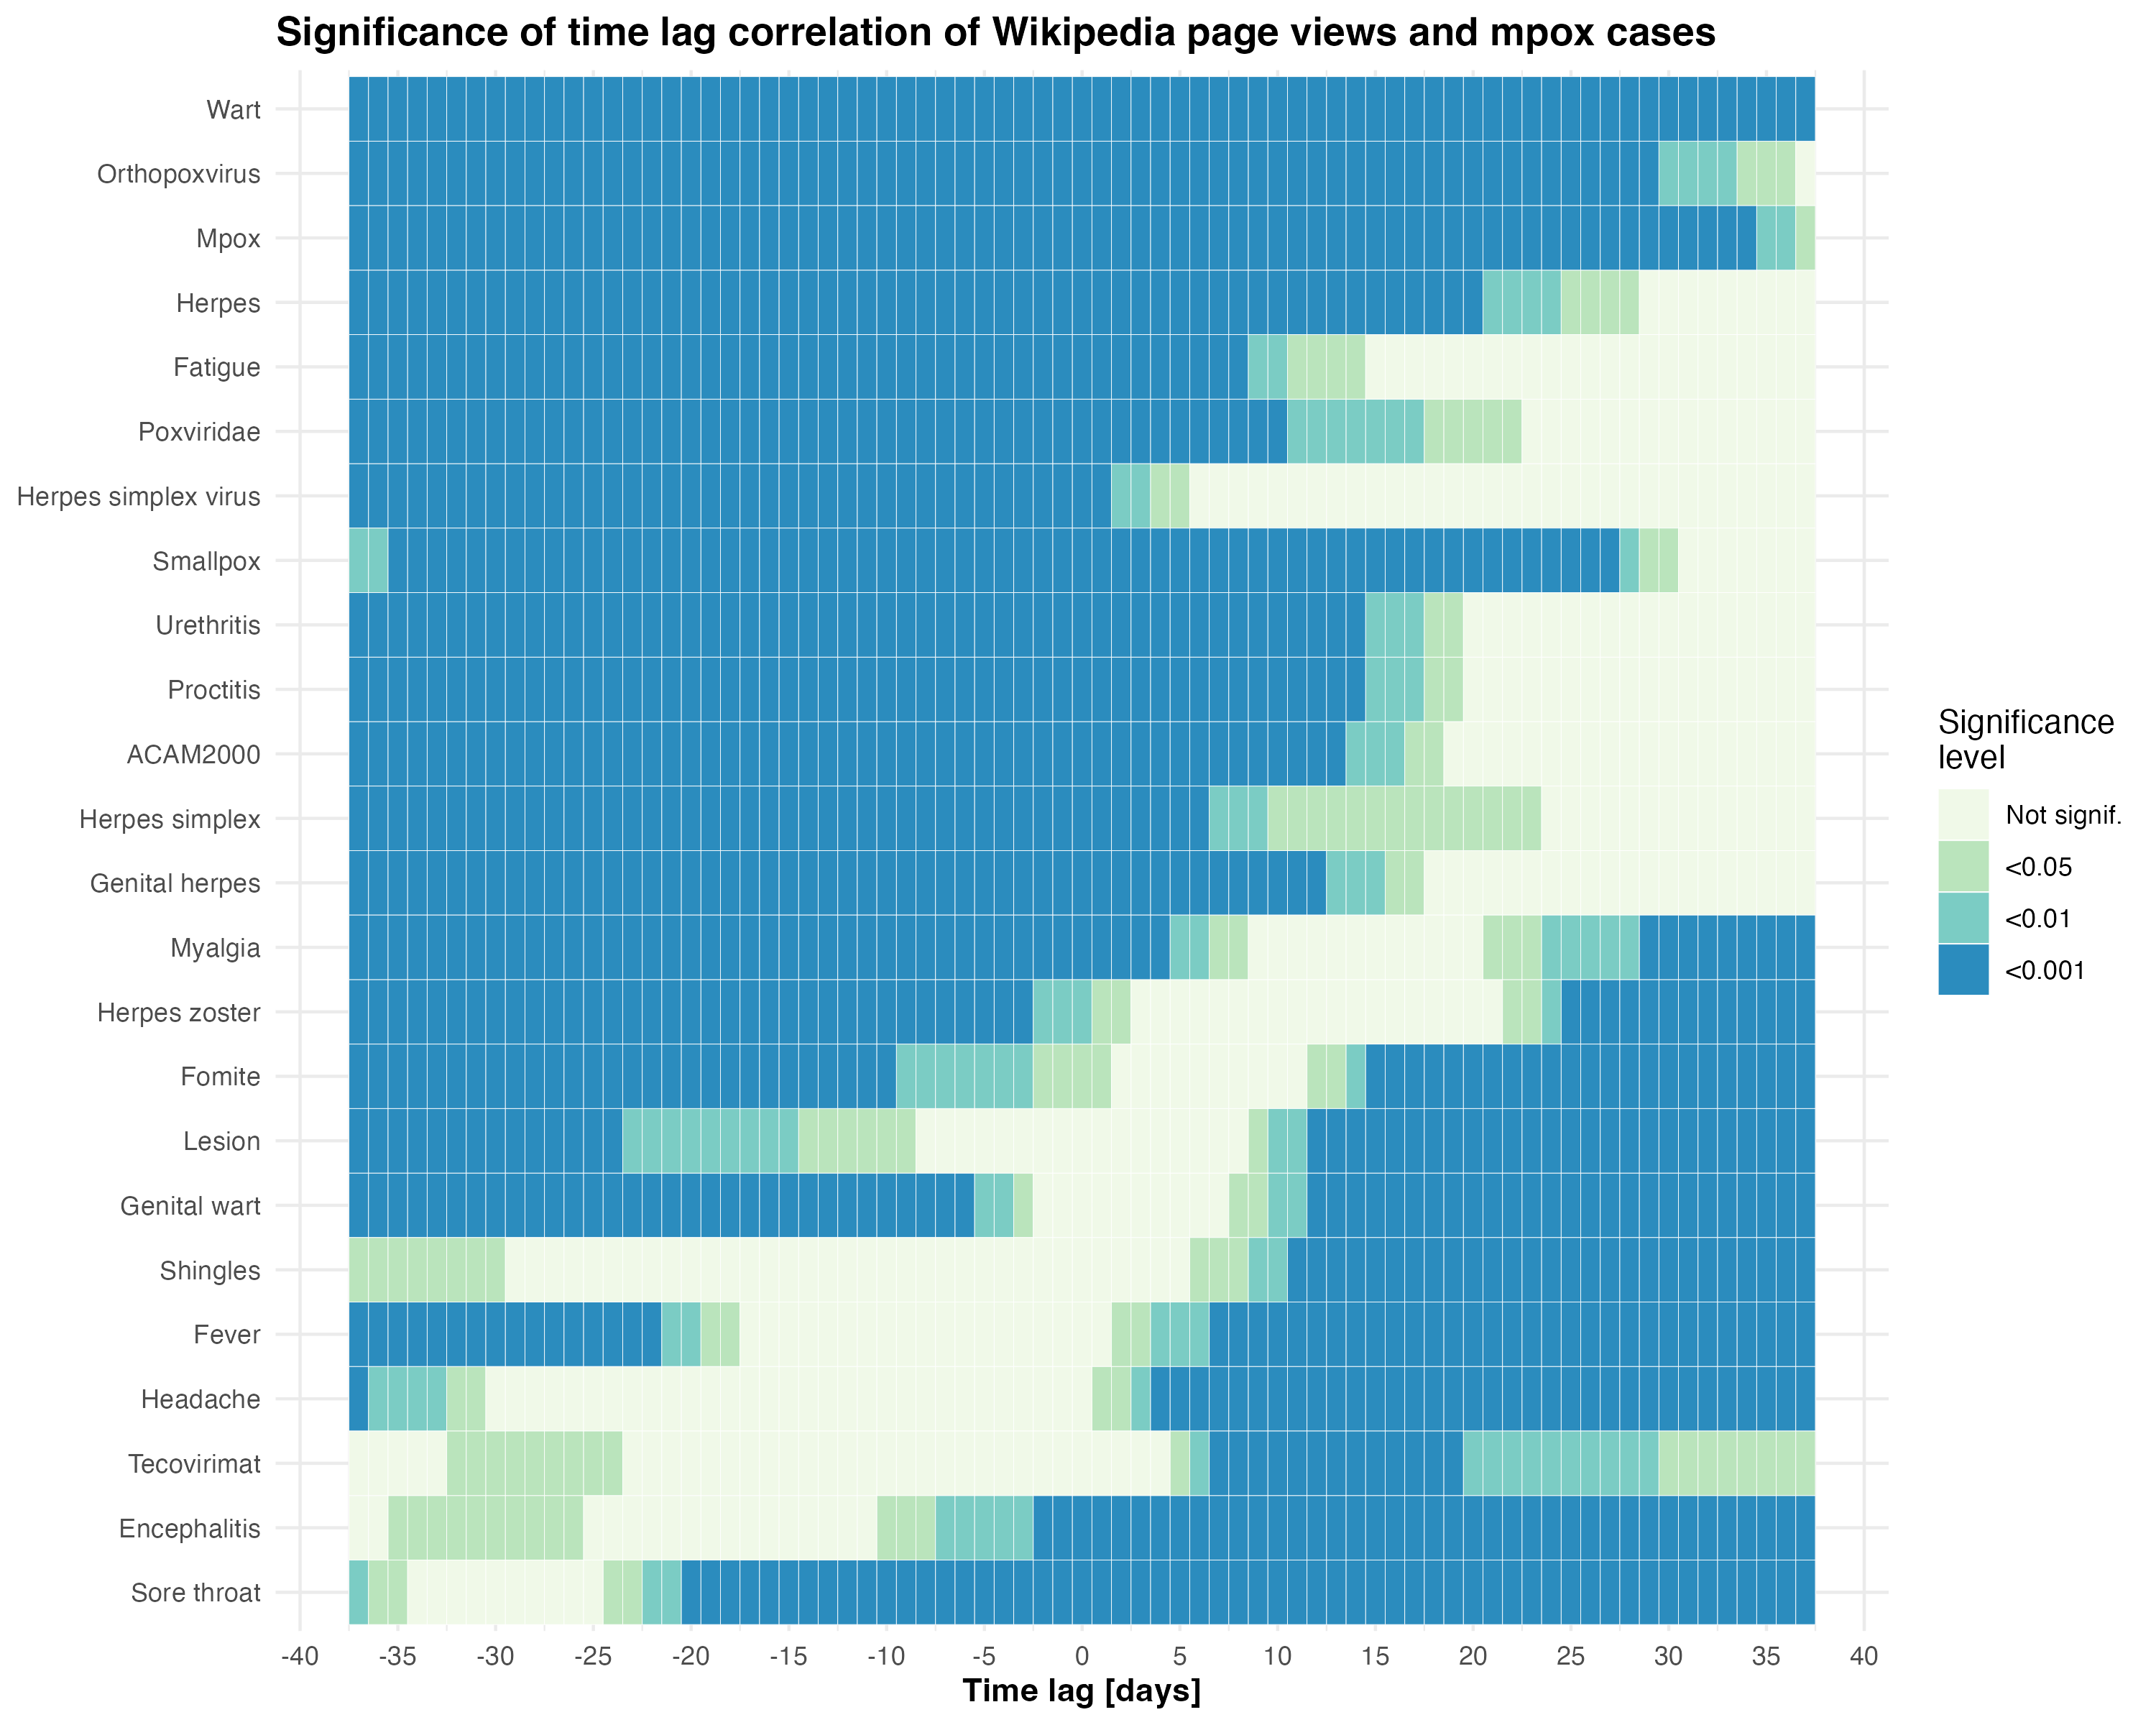
\includegraphics{images/spearman-pvalues-heatmap.png}
\end{center}

\section{Abstract (7) (350 words)}\label{abstract-7-350-words}

{[}To be added last{]}

\(cases_t = \beta_0 + \beta_1 \times pageviews_t + \epsilon_t\)

\section{Introduction (6) (700 words)}\label{introduction-6-700-words}

Google Trends serves as a robust tool for analyzing global search
patterns, providing insights into public interest across countries. This
tool capitalizes on the immense traffic Google receives to evaluate the
popularity of specific keywords over time, measured by Relative Search
Volumes (RSVs). Its ability to offer real-time data on user search
behavior at no cost has made Google Trends a crucial resource in
academic and practical research, including in tracking health-related
public concerns. Google Flu Trends (GFT) is perhaps the most widely
recognized use case, capable of producing highly accurate predictions in
near real-time (\citeproc{ref-ginsberg2009}{Ginsberg et al. 2009}).
Although the accuracy of its predictions were compromised by factors
like media influence during particularly severe outbreaks, as seen
during the 2009 H1N1 pandemic and the severe 2012-2013 flu season, it
succeeded in inspiring others to explore these methods as well
(\citeproc{ref-olson2013}{Olson et al. 2013};
\citeproc{ref-butler2013}{Butler 2013}). Researchers have demonstrated
its utility in predicting cases of diseases such as COVID-19
(\citeproc{ref-abbas2021}{Abbas et al. 2021};
\citeproc{ref-effenberger2020}{Effenberger et al. 2020};
\citeproc{ref-gong2022}{Gong et al. 2022}), malaria
(\citeproc{ref-ocampo2013}{Ocampo, Chunara, and Brownstein 2013}),
norovirus (\citeproc{ref-yuan2021}{Yuan et al. 2021}), and the West-Nile
virus disease (WNVD) (\citeproc{ref-bragazzi2016}{Bragazzi et al. 2016})
among other diseases, highlighting its potential for early outbreak
detection and public health surveillance
(\citeproc{ref-generous2014}{Generous et al. 2014}).

\subsection{Background and Context}\label{background-and-context}

As the world becomes increasingly interconnected and climate change
elevates the risk of zoonotic spillover events, the public becomes ever
more susceptible to global-scale outbreaks
(\citeproc{ref-romanello2021}{Romanello et al. 2021}). In this context,
traditional disease modeling techniques, while effective for
well-documented diseases, may not be as applicable for emerging diseases
with low case numbers and less understood epidemiological parameters.
Critically, public attention plays a pivotal role in disease detection
and response.Problem Definition

A key to outbreak prevention and response is surveillance and detection.
Disease surveillance methodologies encompass a wide range of techniques
used to monitor disease incidence, varying from more traditional
approaches, which often rely on healthcare system reporting, to more
innovative techniques that leverage new technologies and data sources.
The most common form of surveillance relies on healthcare providers
reporting cases of notifiable diseases to public health authorities
{[}SOURCE{]}. Such methods are cost-effective but can suffer from
under-reporting and delays. The problem with these historical methods is
that they require significant time before data become available. This
lag in obtaining accurate and timely data poses a considerable challenge
for policymakers who are tasked with making swift, informed decisions
critical to outbreak containment. The urgency for real-time information
becomes paramount in situations where delays in decision-making can lead
to escalated public health crises. In the face of these challenges, the
vast and continually expanding reservoir of online data presents an
underutilized opportunity for gaining timely insights into disease
dynamics.

\subsection{Proposed Solution}\label{proposed-solution}

The advent of digital tools allows for the real-time tracking of this
attention, offering a valuable complement to established disease
surveillance methods. This is where online attention can serve as an
innovative proxy for tracking disease spread. In this regard, the
2022-2023 multi-country mpox outbreak presents a recent case study,
allowing us to examine the efficacy of real-time data in monitoring a
relatively under-studied disease. By thoroughly exploring these
non-traditional methods, we can more fully understand their advantages
and limitations, thus providing crucial insights for decision-makers.
This research not only enhances our understanding of digital
epidemiology but also contributes to shaping more effective and timely
responses to future infectious disease outbreaks.

\begin{itemize}
\tightlist
\item
  \textbf{Background on the Subject Matter}: While you briefly touch on
  the importance of new disease surveillance methods in the context of
  global interconnectivity and climate change, providing a bit more
  background on traditional vs.~digital epidemiology techniques could
  help set the stage for your study's focus on Wikipedia data.
\end{itemize}

\subsection{Research Questions or
Hypthesis}\label{research-questions-or-hypthesis}

This paper\footnote{Project GitHub repository:
  \url{https://github.com/smkerr/mpox-wiki-analysis}} investigates
whether Wikipedia pageviews can serve as a reliable proxy for public
interest during the 2022-2023 multi-country mpox outbreak. The primary
goal is to assess whether Wikipedia, with its vast user base and
granular data, can effectively serve as a proxy for measuring public
attention and information-seeking behavior in the context of global
health crises. This work is motivated by the limitations of existing
disease modeling techniques for emerging diseases, which may lack
sufficient historical data for accurate forecasting. Public attention,
as measured by digital resources like Wikipedia, could provide early
indicators of disease outbreaks, thus aiding in more timely and
effective public health interventions.

\subsection{Theoretical Framework}\label{theoretical-framework}

\begin{itemize}
\item
  \textbf{Theoretical Framework}: If there's a theoretical framework
  guiding your research, briefly mentioning it in the introduction can
  help readers understand the lens through which you're examining the
  data.

  \begin{itemize}
  \item
    Health Belief Model (HBM)
  \item
    Infodemiology and Infoveillance
  \item
    The Framework of Risk Information Seeking and Processing (RISP)
  \end{itemize}
\end{itemize}

\subsection{Outlook}\label{outlook}

This work contributes to the broader academic discourse by exploring the
potential of open-source data for enhancing disease surveillance and
response strategies. It seeks to validate the efficacy of Wikipedia, as
a non-traditional data source, in providing actionable insights to
policymakers during public health emergencies. In doing so, this work
addresses gaps in the literature regarding the effectiveness of digital
tools in enhancing disease surveillance.

\begin{itemize}
\tightlist
\item
  \textbf{Significance of the Study}: Briefly highlight why this
  research is important. You've mentioned how it contributes to
  understanding digital epidemiology, but expanding on the implications
  for public health policy and emergency response could make a stronger
  case for the study's relevance.
\end{itemize}

\section{Literature Review (5) (1,000
words)}\label{literature-review-5-1000-words}

\begin{itemize}
\item
  \textbf{Objective}: Clearly state the purpose of the Literature Review
  within the context of your thesis.
\item
  \textbf{Scope}: Define the scope of the review, including the time
  frame, geographic focus, and types of sources considered.
\item
  \textbf{Definitions and Concepts}: Introduce and define key theories,
  models, or conceptual frameworks that underpin your research area.
\item
  \textbf{Relevance}: Discuss how these theoretical foundations inform
  the existing research and your study.
\item
  \textbf{Thematic Organization}: Divide the literature into themes or
  categories relevant to your research question. For each theme:

  \begin{itemize}
  \item
    \textbf{Summary}: Provide an overview of the key findings,
    methodologies, and conclusions.
  \item
    \textbf{Critical Analysis}: Evaluate the methodologies used, discuss
    the findings, and note any inconsistencies or debates within the
    theme.
  \item
    \textbf{Connection to Your Research}: Explain how each theme relates
    to your research question or objectives.
  \end{itemize}
\end{itemize}

\begin{itemize}
\item
  \textbf{Overview of Methods}: If relevant, discuss the different
  methodologies employed in the literature, highlighting the evolution
  of research techniques over time.
\item
  \textbf{Strengths and Limitations}: Critically assess the strengths
  and limitations of various approaches.
\item
  \textbf{Identification of Gaps}: Identify areas that have not been
  thoroughly explored or questions that remain unanswered.
\item
  \textbf{Opportunities for Further Research}: Explain how your research
  aims to address these gaps or contribute new insights.
\item
  \textbf{Recent Developments}: Highlight recent studies or emerging
  trends in the field.
\item
  \textbf{Theoretical or Methodological Innovations}: Discuss any new
  theories or methodologies that are gaining traction.
\item
  \textbf{Synthesis}: Summarize the key findings and debates covered in
  the review.
\item
  \textbf{Relevance to Your Study}: Reiterate how the reviewed
  literature supports, contradicts, or informs your research.
\item
  \textbf{Research Question/Hypothesis Revisited}: Optionally, refine or
  reaffirm your research question or hypothesis based on the literature
  review.
\end{itemize}

Several key academic papers lay the groundwork for this approach. In
\href{https://doi.org/10.2196/26331}{``Assessing Public Interest Based
on Wikipedia's Most Visited Medical Articles During the SARS-CoV-2
Outbreak: Search Trends Analysis''} by Chrzanowski et al.~(2021), the
authors investigates how public interest in medical topics changed
during the COVID-19 pandemic, as reflected by Wikipedia pageviews. The
study conducted a retrospective analysis of access to medical articles
across nine language versions of Wikipedia and correlated these patterns
with global and regional COVID-19 deaths, comparing observed data to a
forecast model trained on data from 2015-2019. This involved collecting
daily page view statistics for 37,880 articles curated by the English
Wikipedia Medicine Project from 1 July 2015 to 13 September 2020. The
authors sourced page view statistics using ToolForge, a page view
analytics tool) and sourced COVID-19 death statistics from Our World in
Data. It found a correlation between the pandemic's severity and
pageviews for COVID-19--related Wikipedia articles, concluding that
changes in article popularity could serve as a method for
epidemiological surveillance by reflecting public attention during
disease outbreaks. Furthermore, it demonstrates the potential for using
Wikipedia data for epidemiological surveillance and understanding public
information-seeking behavior during disease outbreaks. While the paper
focuses on the COVID-19 pandemic, similar methodologies can be applied
to provide insights into public attention and information-seeking
behavior during the Mpox outbreak.

\href{https://doi.org/10.1002\%2Fjmv.28382}{``Association between public
attention and monkeypox epidemic: A global lag-correlation analysis''}
by Yan et al.~(2023) investigates the association between public
attention, as measured by Google Trends Index (GTI), and the global mpox
oubtreak. The authors use Google Trends data for information on internet
search activity related to mpox as well as data on daily confirmed mpox
cases from Our World in Data. It tests time-lag correlations between GTI
and daily confirmed mpox cases across the 20 countries with the highest
case numbers as of 20 September 2022 using the Spearman correlation
coefficients, over a range of -36 to +36 days. Spearman correlation
coefficients from these 20 countries were pooled to provide a combined
correlation coefficient for each lag. To test whether the time series
was stationary, an Augment Dickey-Fuller (ADF) test is applied. The
study finds a strong positive correlation, particularly noticeable 13
days after a peak in public attention. The study also conducted
meta-analyses and utilized vector autoregression (VAR) models to analyze
the temporal relationship between GTI and daily confirmed mpox cases,
and a Granger-causality test was employed to evaluate whether the GTI
trend could predict daily confirmed mpox cases. The findings suggest
that GTI could be a useful tool for early monitoring and prediction of
mpox cases, highlighting the significance of digital epidemiology in
infectious disease surveillance. The study emphasizes the potential of
internet data like GTI in providing early warning signs for health
outbreaks and aiding in rapid response strategies. While the study
utilizes GTI data to public attention towards the mpox outbreak, however
similar methods can be applied to Wikipedia pageviews data to test
whether the same conclusions can be drawn using Wikipedia as a data
source.

In \href{https://doi.org/10.3390/ijerph20043395}{``Trends in Online
Search Activity and the Correlation with Daily New Cases of Monkeypox
among 102 Countries or Territories''} by Du et al.~(2023), the authors
investigate the relationship between online search activity related to
mpox and the actual daily new cases of mpox across 102 countries or
territories. The study aims to understand how internet search trends can
reflect public awareness towards mpox, potentially serving as an early
indicator for outbreaks. Data on daily mpox cases from 1 May 2022 to 9
October 2022 was sourced from Our World in Data, while online search
activity data related to mpox was sourced from Google Trends using the
keyword ``monkeypox''.\footnote{Note that this study was conducted prior
  to WHO's recommendation that monkeypox instead be referred to as
  ``mpox'' on 28 November 2022:
  \url{https://www.who.int/news/item/28-11-2022-who-recommends-new-name-for-monkeypox-disease}}
Online search activity was expressed as relative normalized search
volume numbers (RNSNs) ranging from 0 to 100 to reflect how many
searches are performed for a keyword relative to the total number of
searches on the internet over time where a value of 100 represents the
time point at which the search term has reached its peak in popularity.
Demographic data including total population, population density, average
years of schooling, socioeconomic status, and public tourism were
sourced from the United Nations and World Bank. Data on health status
including HIV prevalence, sanitation levels, and health workforce
densities were obtained from the 2019 Global Burden of Disease study.
The authors use a segmented time-series analysis to estimate the impact
of the PHEIC declaration on online search activity, adjusting for daily
new cases across 194 countries or territories. Furthermore, the study
tests time-lag correlations between online search activity and daily new
cases, specifically considering lags of -21, -14, -7, 0, +7, +14, and
+21 days. Next, a general linear regression model (GLM) is used to
explore influencing factors on the relationship between online search
activity and daily new cases. The authors find a significant correlation
between online search activity and daily mpox cases, with online
searches often preceding reporting of new cases. This study highlights
the value of integrating internet search data into public health
surveillance for emerging infectious diseases. Similar to the paper by
Yan et al., this study utilizes Google Trends data, however similar
methodologies could be applied towards Wikipedia pageviews data.

Beyond these studies, several other academic papers have contributed
analysis to various aspects of the relationship between online
information-seeking behavior and public health.

\begin{itemize}
\item
  \href{https://doi.org/10.1098/rsos.160460}{García-Gavilanes et
  al.~(2016)} use Wikipedia page view and page edit statistics to
  investigate public attention towards airline crashes.
\item
  In their analysis of page views for COVID-19-related Wikipedia pages,
  \href{https://doi.org/10.2196/21597}{Gozzi et al.~(2020)} find that
  page views were mainly driven by media coverage, declined rapidly,
  even while COVID-19 incidence remained high, raising questions about
  the impacts of attention saturation in disease outbreak settings.
\item
  \href{https://doi.org/10.3390/info14010005}{Bhagavathula and
  Raubenheimer (2023)} conducted a joinpoint regression analysis to
  measure hourly percentage changes (HPC) in search volume in the hours
  immediately preceding and following WHO's determination to assign
  PHEIC status to mpox, finding an overall increase in
  information-seeking behavior, although results varied by country. This
  study revealed a 103\% increase in public interest in top five
  Mpox-affected countries immediately following the WHO PHEIC
  announcement. However, search interest waned after the announcement,
  so that search interest appeared to reflect media attention more than
  disease spread.
\item
  \href{https://doi.org/10.3389/fpubh.2021.755530}{Gong et al.~(2022)}
  use the Baidu Index (BDI) and Sina Macro Index (SMI) to investigate
  the association between public attention towards the COVID-19 pandemic
  and new cases using Spearman correlation.
\item
  \href{https://doi.org/10.3390/ijerph18094560}{Abbas et al.~(2021)}
  analyze associations between Google Search Trends for symptoms of
  COVID-19 and confirmed cases and deaths within the United States,
  demonstrating abilitiy to predict cases up to three weeks prior.
\item
  \href{https://doi.org/10.1371/journal.pcbi.1004239}{Hickmann et
  al.~(2015)} demonstrate that it is possible to use Wikipedia page view
  statistics and CDC influenza-like illness (ILI) reports to create a
  weekly forecast for seasonal influenza, finding that that Wikipedia
  article access are highly correlated with historical ILI records,
  allowing for highly accurate disease forecasts several weeks before
  case data is available.
\end{itemize}

Given the existing literature, this thesis aims to fill the research gap
by investigating whether Wikipedia can be predictive of mpox cases
during the 2022-2023 multi-country outbreak. While previous studies have
evaluated Wikipedia data for COVID-19 and others have utilized Google
Trends data for mpox, this thesis represents the first attempt, as far
as I am aware, to explore the relationship between Wikipedia page view
statistics and mpox cases.

\section{Theory / Research Questions and Hypotheses (1) (1,000
words)}\label{theory-research-questions-and-hypotheses-1-1000-words}

\begin{itemize}
\item
  \textbf{Rationale}: Begin by explaining why the chosen theoretical
  framework is suitable for your research, linking it to the gaps or
  issues identified in the literature review.
\item
  \textbf{Description}: Provide a detailed description of the
  theoretical framework or models you'll be using, including key
  concepts, variables, and the relationships between them.
\item
  \textbf{Relevance}: Discuss how this framework has been applied in
  previous research and its significance in addressing your research
  problem.
\item
  \textbf{Definitions}: Clearly define the main constructs or variables
  within your theoretical framework, ensuring they are specific to your
  study's context.
\item
  \textbf{Operationalization}: Explain how you will measure these
  constructs or variables in your research, making theoretical concepts
  tangible and researchable.
\item
  \textbf{Research Questions}:

  \begin{itemize}
  \item
    If your study is more exploratory or qualitative, list the research
    questions that guide your investigation. Each question should be
    clearly formulated to explore the relationships or phenomena
    described by your theoretical framework.
  \item
    \textbf{Purpose}: Clarify what each question aims to discover or
    understand about the relationship between variables or concepts.
  \end{itemize}
\item
  \textbf{Hypotheses}:

  \begin{itemize}
  \item
    For more quantitative or confirmatory studies, formulate specific
    hypotheses. These are predictive statements about the expected
    relationships between variables based on your theoretical framework.
  \item
    \textbf{Directionality}: Indicate whether each hypothesis is
    directional (specifying the nature of the relationship) or
    non-directional (simply stating that a relationship exists).
  \end{itemize}
\item
  \textbf{Theoretical Justification}: Provide a rationale for each
  research question or hypothesis, drawing on your theoretical framework
  and findings from the literature review.
\item
  \textbf{Research Gap}: Demonstrate how your questions or hypotheses
  address a gap in the existing literature or contribute to a deeper
  understanding of the topic.
\end{itemize}

\begin{itemize}
\item
  \textbf{Methodological Implications}: Briefly discuss how your
  research questions or hypotheses will influence your choice of
  research design, methods of data collection, and analysis techniques.
\item
  \textbf{Feasibility and Limitations}: Acknowledge any limitations that
  your theoretical framework or hypotheses may impose on your study and
  how you plan to address them.
\item
  \textbf{Summary}: Conclude by summarizing the key points made in this
  section, reinforcing the importance of your theoretical framework and
  research questions/hypotheses in guiding your study.
\item
  \textbf{Transition}: Provide a smooth transition to the next section
  of your thesis, typically the methodology, indicating how the theory
  will be applied to empirical research.
\end{itemize}

To what extent can Wikipedia data be effectively utilized as an
alternative method for measuring public attention and
information-seeking behavior during the 2022-2023 multi-country mpox
outbreak?

This research question engages the following current and relevant
conversations within the literature:

\begin{itemize}
\item
  \emph{Open Source Data for Public Health Surveillance}: Examining the
  utility and limitations of using public data sources like Wikipedia to
  monitor and assess public health events, contributing to ongoing
  discussions about their reliability and relevance.
\item
  \emph{Information Dissemination and Public Awareness}: Investigating
  the extent to which public awareness of outbreaks is shaped by the
  impact (number of cases and/or deaths), connecting with debates about
  information ecosystems and their impact on public health
  communication.
\item
  \emph{Policy Implications}: Discussing the potential policy
  recommendations and interventions that can arise from a better
  understanding of public attention and information-seeking behavior
  during outbreaks on digital platforms.
\end{itemize}

My thesis also contains several sub-questions to be investigated in
support of the main research question:

\begin{itemize}
\item
  Which medical articles saw traffic volume increase significantly after
  the start of the mpox outbreak?
\item
  To what extent do the number of mpox cases correlate with the traffic
  volume of mpox-related Wikipedia articles?
\item
  How effective is Wikipedia analytics data compared to other data
  sources (e.g., Google Trends) when it comes to gauging public
  attention towards the mpox outbreak?
\end{itemize}

\section{Data and Methods (2)}\label{data-and-methods-2}

\begin{itemize}
\tightlist
\item
  \textbf{Overview}: Start with a brief introduction that outlines the
  purpose of this section, connecting it back to your research questions
  or hypotheses.
\end{itemize}

\subsection{Data sources (700 words)}\label{data-sources-700-words}

\begin{itemize}
\item
  \textbf{Data Source(s)}: Describe where your data comes from. For
  example, mention if you used datasets from public repositories,
  conducted surveys, or collected observational data. Provide the
  context and justification for choosing these sources.
\item
  \textbf{Sample Selection}: Detail how you selected your sample.
  Include information on the population of interest, sampling frame, and
  any sampling techniques used (e.g., random sampling, stratified
  sampling).
\item
  \textbf{Data Collection Procedures}: Explain how the data were
  collected, including any instruments or tools used (e.g., survey
  questionnaires, interview guides).
\item
  \textbf{Data Description}: Provide a descriptive overview of your
  data, including the size of the dataset, key variables, and any
  pertinent characteristics of the data relevant to your research
  questions.
\end{itemize}

To answer my research question, I will rely on two main data sources.
First, country-level data on the weekly number of mpox cases is sourced
from WHO.\footnote{\url{https://worldhealthorg.shinyapps.io/mpx_global/}}
Second, Wikipedia analytics data on daily page view volume by article is
sourced directly from Wikipedia.\footnote{\url{https://wikitech.wikimedia.org/wiki/Data_Engineering/Systems/AQS}}

My topic focuses on assessing public attention towards the 2022-2023
multi-country mpox outbreak using Wikipedia data. As such, this analysis
relies on two main data sources. First, country-level data on the weekly
number of mpox cases is sourced from the World Health Organization
(WHO). Second, Wikipedia analytics data on page view volume is sourced
directly from Wikipedia.

Data on the number of confirmed mpox cases is obtained from the World
Health Organization (WHO), while page view statistics for Wikipedia
articles related to mpox are sourced directly from Wikipedia. The
analysis is restricted to the 10 countries most affected by the
outbreak, using time series analysis and lag-correlation methods to
examine the relationship between Wikipedia page views and mpox case
numbers. The study aims to identify patterns and correlations that could
support the use of Wikipedia data as a predictive tool for public health
surveillance.

\subsubsection{Mpox case data}\label{mpox-case-data}

\begin{itemize}
\item
  \textbf{Methodological Approach}: Outline the methodological approach
  or approaches you used in your study (e.g., qualitative, quantitative,
  mixed methods). Explain why this approach is suitable for addressing
  your research questions or testing your hypotheses.
\item
  \textbf{Data Preparation}: Describe any procedures used to prepare the
  data for analysis, such as data cleaning, coding, or the handling of
  missing data.
\item
  \textbf{Analytical Techniques}: Detail the specific analytical
  techniques or statistical methods used to analyze the data. Include
  information on any software or tools used in the analysis.
\item
  \textbf{Validation Methods}: If applicable, discuss how you validated
  your findings. This might involve techniques such as cross-validation,
  reliability and validity testing of instruments, or triangulation of
  data sources.
\end{itemize}

Daily aggregated numbers of mpox cases by country correspond with the
date on which cases were reported to public health authorities. One
advantage of this dataset is that it is considered to be largely
complete since it comprises every confirmed and probable case reported
to the national public health authorities.\footnote{For more information
  on what constitutes a confirmed or probable case, please refer to
  WHO's mpox case definitions:
  \url{https://www.who.int/emergencies/outbreak-toolkit/disease-outbreak-toolboxes/mpox-outbreak-toolbox}}
While this still leaves room for cases to go underreported in instances
where an individual does not seek medical attention (e.g., for fear of
stygmatization) or for asymptomatic cases, it still represents the most
comprehensive view of the outbreak's scale. Aggregated data is available
for all reported cases as of 31 December 2023.

The top 10 countries by number of confirmed cases are the United States
of America (31,246), Brazil (10,967), Spain (7,752), France (4,171),
Colombia (4,090), Mexico (4,078), the United Kingdom (3,875), Peru
(3,812), Germany (3,800), and China\footnote{Cases shown include those
  reported in mainland China (1,611), Taiwan (333), Hong Kong (80), and
  Macao (1).} (2,025).

As of 31 December 2023, mpox cases have been reported by 117 WHO Member
States across all six WHO regions. The dataset contains cases reported
between 7 January 2022 to 31 December 2023.

For this analysis, I will only consider confirmed cases. However, I do
not expect this decision to greatly impact the results considering that
probable cases only make up 0.7\% of overall cases (652/93,682) and only
eight countries report any probable cases. While Puerto Rico reports the
highest proportion of probable cases at 42\% of total cases (150/361),
probable cases make up less than 5\% of the remaining countries' total
cases.

While WHO collects aggregated data on a daily basis, nearly all
countries' public health authorities report cases at a weekly frequency.
As a result, it is more useful to aggregate cases by epidemic week. The
epidemic curve below depicts the aggregated weekly number of cases by
week reported.

While the global trend appears to have been quite coherent with the
number of weekly cases peaking in July 2022, this disguises the fact
that the trends in cases looked quite distinct at the WHO region-level.

Here we observe that there is substantial variation between the six WHO
regions, with the Eastern Mediterranean Region, European Region, and
Region of the Americas following a similar trend with cases peaking in
summer/fall 2022, while cases in the South-East Asia Region and Western
Pacific Region peak in summer/fall 2023. In contrast, cases reported by
the African Region appear to be more uniformly distributed, reflecting
the fact that mpox is endemic to certain areas of western and central
Africa.

In addition to aggregated case data, WHO also collects line list data
where each row corresponds with an individual case and contains
information on demographics, clinical presentation, epidemiological
exposure factors, and laboratory testing.\footnote{\url{https://www.who.int/publications/m/item/monkeypox-minimum-dataset-case-reporting-form-(crf)}}
Due to privacy concerns, line list data is stripped of all personally
identifiable information and aggregated by country and date before being
made available by WHO.\footnote{\url{https://worldhealthorg.shinyapps.io/mpx_global/}}
In contrast to aggregated case data, the \texttt{date} variable of the
detailed case dataset corresponds with either the date of symptom onset,
the date of diagnosis (if date of symptom onset is not available), or
the date of reporting (if date of symptom onset and date of diagnosis
are not available).\footnote{\url{https://worldhealthorg.shinyapps.io/mpx_global/}}
This difference in how cases are assigned to a date grants us a much
more granular view of countries' epidemic curves, as shown below. Dates
are aggregated at the weekly level to further protect individual cases'
privacy.

A significant disadvantage of this detailed dataset is that it only
contains information 63\% for all reported mpox cases (58,883/93,030).
This is driven almost entirely by the fact that WHO no longer includes
cases from the United States in this dataset, despite the fact that the
United States represents 34\% of global cases (31,246/93,030). That
said, this data can still be useful for analysis of other countries. As
such, detailed dataset can complement the aggregated data presented
above.

While WHO collects line list data on a daily basis, this data is
aggregated by epidemic week to safeguard the privacy of individual
cases. The epidemic curve below depicts the weekly number of cases.
Compared to the epidemic curves produced using aggregated data, the
detailed data allows us to plot much smoother curves which seem to
adhere more closely to the trend we might expect of an infectious
disease outbreak.

Again, while the global trend appears to have been quite coherent with
the number of weekly cases peaking in July 2022, the trends vary at the
WHO region-level.

\subsubsection{Wikipedia data}\label{wikipedia-data}

The Wikimedia Foundation makes it straightforward to access various
analytics data related to its projects, including Wikipedia, by
providing the
\href{https://wikitech.wikimedia.org/wiki/Data_Engineering/Systems/AQS}{Wikimedia
Analytics Query Service (AQS)}
\href{https://wikimedia.org/api/rest_v1/}{REST API}. AQS offers a range
of analytics data, such as page view statistics, editor activity levels,
and other traffic data from as far back as 1 August 2015. The REST API
facilitates the retrieval of analytics data from Wikipedia in a
structured way. Given that Wikipedia data is abundant, publicly
accessible, and commonly used, many resources exist to easily access
this data.\footnote{Mikhail Popov, Data Science Manager in Product
  Analytics at the Wikimedia Foundation, has published a list of R
  packages related to or affiliated with the Wikimedia Foundation here:
  \url{https://people.wikimedia.org/~bearloga/notes/r-pkgs.html}}
\{\href{https://wikimedia.github.io/waxer/}{waxer}\} is one such package
which serves as a Wikimedia API wrapper that facilitates querying for
traffic (pageviews, unique devices), user (e.g.~active editors), and
content-based metrics (e.g.~edits counts, pages counts) from Wikimedia
Analytics Query Service with R.

Since this project is concerned with assessing public attention,
Wikipedia page view statistics will serve as our primary measure for
online information-seeking behavior. We query page view statistics from
the AQS REST API using the following specifications:

We start exploring the dataset by examining the absolute and relative
frequency of different values within the \texttt{project} and
\texttt{page\_name} variables. As expected, all page views are for the
English Wikipedia project. Notably, the ``Mpox'' article has a
substantially higher traffic volume than the ``Monkeypox virus'' article
(71\% vs.~29\%).

Next, we explore the missingness of each of variable in the
\texttt{pageviews} dataset. We find that \texttt{redirect\_name} is the
only column missing values. For the specified Wikipedia project and
articles, 27\% of page views were redirected from other search terms.

Seeing as a substantial number of page views are driven by redirects, it
is important to understand whether it is valid to include these
redirects in our analysis. If search terms appear related to mpox or the
monkeypox virus, then it is safe to assume that this represents online
information-seeking behavior towards our topic. Our table shows that all
search appear to directly relate to mpox or the monkeypox virus, so we
conclude that is valid to include redirects in this analysis. This will
be reevaluated and handled as more projects and articles are added to
the analysis.

Considering that mpox case data is available at a weekly level of
granularity, we aggregate page view data by week and plot the results
below. We observer two large spikes, with the first centered on May 2022
when non-endemic countries began reporting mpox cases\footnote{\url{https://www.who.int/emergencies/situations/monkeypox-oubreak-2022}}
and the second centered on late July 2022 when WHO declared mpox to be a
Public Health Emergency of International Concern (PHEIC).\footnote{\url{https://www.who.int/europe/news/item/23-07-2022-who-director-general-declares-the-ongoing-monkeypox-outbreak-a-public-health-event-of-international-concern}}
Other smaller peaks can be observed, although the general trend
indicates that public attention decreases over time.

Another element of this project involves developing a baseline for what
online information-seeking behavior may have looked like in the absence
of the mpox outbreak, as measured by Wikipedia article access. For this,
we will use overall project views for the respective Wikipedia projects
to detect seasonality and long-term trends in Wikipedia search trends.
To illustrate what this looks, we examine the Wikipedia projects
corresponding with the most common languages in the top 10 countries by
number of mpox cases.

The plot below shows that English Wikipedia predominates overall
Wikipedia traffic, with weekly traffic levels for the other language
projects clustered together well below.

While this Data Report showcases the underlying data structure of
Wikipedia page view statistics using as ``Mpox'' and ``Monkeypox virus''
articles as mere examples, there are many other articles related to mpox
and its symptoms\footnote{\url{https://www.who.int/news-room/fact-sheets/detail/monkeypox}}
that may also contribute to this analysis. Supplemental article titles
are listed below. Since article titles have been recorded in English,
the next step would be to cross-reference them with their corresponding
titles for other Wikipedia projects.

\subsection{Methods (1,000 words)}\label{methods-1000-words}

While mpox case data is available for 117 WHO Member States and
Wikipedia page view statistics exist for nearly 300 languages, I will
limit the scope of this analysis to the 10 countries with the most
cumulative cases, including the United States of America (31,246),
Brazil (10,967), Spain (7,752), France (4,171), Colombia (4,090), Mexico
(4,078), the United Kingdom (3,875), Peru (3,812), Germany (3,800), and
China\footnote{Cases shown include those reported in mainland China
  (1,611), Taiwan (333), Hong Kong (80), and Macao (1).} (2,025).
Accordingly, I will limit the analysis to the Wikipedia projects for the
languages that prominently feature in these countries, including English
(the United States of America and the United Kingdom), Portuguese
(Brazil), Spanish (Spain, Mexico, and Peru), French (France), German
(Germany), Chinese (China). I will examine the time period from 1
January 2022 to 31 December 2023.

\begin{longtable}[]{@{}
  >{\raggedright\arraybackslash}p{(\columnwidth - 4\tabcolsep) * \real{0.3714}}
  >{\raggedright\arraybackslash}p{(\columnwidth - 4\tabcolsep) * \real{0.3000}}
  >{\raggedright\arraybackslash}p{(\columnwidth - 4\tabcolsep) * \real{0.3286}}@{}}
\toprule\noalign{}
\begin{minipage}[b]{\linewidth}\raggedright
\textbf{Country}
\end{minipage} & \begin{minipage}[b]{\linewidth}\raggedright
\textbf{Number of cases}
\end{minipage} & \begin{minipage}[b]{\linewidth}\raggedright
\textbf{Wikipedia project}
\end{minipage} \\
\midrule\noalign{}
\endhead
\bottomrule\noalign{}
\endlastfoot
United States of America & 31,246 & English \\
Brazil & 10,967 & Portuguese \\
Spain & 7,752 & Spanish \\
France & 4,171 & French \\
Colombia & 4,090 & Spanish \\
Mexico & 4,078 & Spanish \\
United Kingdom & 3,875 & English \\
Peru & 3,812 & Spanish \\
Germany & 3,800 & German \\
China & 2,025 & Chinese \\
\end{longtable}

My proposed methodology takes inspiration from th work of
\href{https://doi.org/10.1002\%2Fjmv.28382}{Yan et al.} and
\href{https://doi.org/10.3390/ijerph20043395}{Du et al.} I will conduct
an observational study to assess the lag-correlation between public
attention and mpox cases for the 10 countries with the most cumulative
cases.

\begin{enumerate}
\def\labelenumi{\arabic{enumi}.}
\tightlist
\item
  Define collection of mpox-related Wikipedia articles

  \begin{itemize}
  \tightlist
  \item
    Identify articles directly related to mpox, including historical
    information, symptoms, treatment, and prevention.
  \item
    Identify articles with a low degree of separation within network of
    Wikipedia articles.
  \item
    Analyze Wikipedia page view statistics to identify medical articles
    that experienced significant increases in traffic coinciding with
    the timeline of the 2022-2023 mpox outbreak.\footnote{An assessment
      would need to be made to determine that the increase in traffic
      volume of certain medical articles following the start of the
      outbreak is not spurious but substantial.}
  \end{itemize}
\item
  Data preparation

  \begin{itemize}
  \tightlist
  \item
    Collect daily mpox case numbers from WHO.
  \item
    Extract daily traffic volume data for the defined collection of
    Wikipedia articles using Wikipedia's API with the \{waxer\} package
    using R.
  \item
    De-noise data by aggregating both mpox cases and Wikipedia page view
    statistics to the weekly level.
  \item
    Standardize Wikipedia traffic volumes to be expressed as a
    percentage of total traffic volume for a given Wikipedia language
    version.
  \end{itemize}
\item
  Statistical analysis

  \begin{itemize}
  \tightlist
  \item
    Perform Spearman correlation tests to examine the time-lag
    relationship between Wikipedia traffic volumes and mpox case
    numbers. The range of -21 to +21 days will allow analysis of lead
    and lag effects.
  \item
    Use non-parametric methods, considering the non-normal distribution
    of the data.
  \end{itemize}
\item
  Augmented Dickey-Fuller (ADF) test

  \begin{itemize}
  \tightlist
  \item
    Implement the ADF test to check for stationarity in both the
    Wikipedia traffic and mpox case series. Non-stationary data can lead
    to spurious results in subsequent analyses.
  \end{itemize}
\item
  Vector autoregression (VAR) model

  \begin{itemize}
  \tightlist
  \item
    Develop a VAR model to understand the dynamic relationship between
    the two time series. This model will help in capturing the temporal
    interdependencies and feedback mechanisms between Wikipedia traffic
    and mpox cases.
  \item
    Determine the optimal lag length for the VAR model based on
    information criteria like AIC or BIC.
  \end{itemize}
\item
  Granger causality test

  \begin{itemize}
  \tightlist
  \item
    Apply the Granger causality test within the VAR framework to assess
    whether Wikipedia traffic volumes can be considered a predictor of
    mpox case trajectories.
  \item
    This test will help determine if changes in Wikipedia page views
    precede changes in mpox cases, indicating a predictive relationship.
  \end{itemize}
\item
  Validation and robustness checks

  \begin{itemize}
  \tightlist
  \item
    Conduct sensitivity analyses to test the robustness of the findings
    against different model specifications and subsets of data.
  \item
    Validate the results through comparison with other studies or
    datasets.
  \end{itemize}
\item
  Interpretation and implications

  \begin{itemize}
  \tightlist
  \item
    Interpret the results, while considering the limitations of
    observational data and the potential for confounding factors.
  \item
    Discuss the implications for public health surveillance during
    health emergencies.
  \end{itemize}
\end{enumerate}

\subsection{Ethical considerations}\label{ethical-considerations}

\begin{itemize}
\tightlist
\item
  \textbf{Data Privacy}: Discuss measures taken to ensure the privacy
  and confidentiality of participant data.
\end{itemize}

\subsection{Limitations of Data and
Methods}\label{limitations-of-data-and-methods}

\begin{itemize}
\item
  \textbf{Acknowledgment of Limitations}: Clearly outline any
  limitations or biases inherent in your data or methodological approach
  that could affect your results or the generalizability of your
  findings.
\item
  \textbf{Mitigation Strategies}: Describe any steps taken to mitigate
  the impact of these limitations.
\end{itemize}

\subsection{Conclusion}\label{conclusion}

\begin{itemize}
\item
  \textbf{Summary}: Conclude this section by summarizing the key points
  about your data and methods, emphasizing their appropriateness and
  robustness in addressing your research questions.
\item
  \textbf{Transition to Results}: Provide a smooth transition to the
  next section of your thesis, which will typically present the results
  of your analysis.
\end{itemize}

\section{Analysis (3) (1,400 words)}\label{analysis-3-1400-words}

\begin{itemize}
\tightlist
\item
  \textbf{Brief Overview}: Start with a short paragraph introducing the
  Analysis section. Highlight the analytical methods used (descriptive
  analysis and regression models) and their relevance to your research
  question
\end{itemize}

\subsection{Descriptive analysis}\label{descriptive-analysis}

\begin{itemize}
\item
  \textbf{Purpose and Overview}: State the purpose of conducting a
  descriptive analysis. This may involve summarizing the main
  characteristics of the data, establishing patterns, or identifying
  trends.
\item
  \textbf{Presentation of Findings}:

  \begin{itemize}
  \item
    Use tables, charts, and graphs to present key statistics such as
    means, medians, modes, ranges, and standard deviations.
  \item
    Describe significant findings from these visual and statistical
    summaries, referring to the variables of interest in your study.
  \end{itemize}
\item
  \textbf{Interpretation}: Provide a narrative interpretation of the
  descriptive statistics and what they reveal about the dataset's
  underlying patterns or trends.
\item
  \textbf{Link to Research Questions}: Explain how the descriptive
  analysis contributes to answering your research questions or setting
  the stage for further analysis.
\end{itemize}

\subsection{Regression models}\label{regression-models}

\begin{itemize}
\item
  \textbf{Rationale for Using Regression Models}: Explain why regression
  models are appropriate for your study. Discuss how they can help
  explore the relationships between variables or predict outcomes based
  on your theoretical framework.
\item
  \textbf{Model Specification}:

  \begin{itemize}
  \item
    Describe the type(s) of regression model(s) used (e.g., linear
    regression, logistic regression) and why they were chosen.
  \item
    Detail the dependent and independent variables, including any
    control variables, and the rationale for their selection.
  \end{itemize}
\item
  \textbf{Assumptions and Preliminary Tests}: Briefly mention any
  assumptions underlying the regression models and describe any
  preliminary tests conducted to ensure these assumptions were met
  (e.g., tests for multicollinearity, normality, homoscedasticity).
\item
  \textbf{Presentation of Regression Results}:

  \begin{itemize}
  \item
    Present the results of the regression analysis in a clear and
    organized manner, using tables to summarize the model coefficients,
    significance levels, and fit statistics (e.g., R-squared, AIC).
  \item
    Highlight key findings from the regression analysis, focusing on the
    relationship and significance of the independent variables in
    predicting the dependent variable(s).
  \end{itemize}
\item
  \textbf{Interpretation of Results}:

  \begin{itemize}
  \item
    Interpret the coefficients, explaining the meaning of the
    significant predictors in the context of your research questions.
  \item
    Discuss the implications of the findings, considering the strength,
    direction, and significance of the relationships found.
  \end{itemize}
\item
  \textbf{Model Fit and Validation}: Comment on the overall fit and
  robustness of the regression models. Mention any model validation
  techniques used (e.g., cross-validation, out-of-sample prediction).
\end{itemize}

\subsection{Synthesis and link to Hypothesis / Research
Questions}\label{synthesis-and-link-to-hypothesis-research-questions}

\begin{itemize}
\item
  \textbf{Synthesizing Findings}: Draw connections between the
  descriptive analyses and regression model outcomes. Discuss how these
  analyses collectively address your research questions or
  support/refute your hypotheses.
\item
  \textbf{Insights and Implications}: Provide insights gained from the
  analysis, emphasizing their implications for the theoretical
  framework, existing literature, and practical applications.
\item
  \textbf{Summary of Key Findings}: Summarize the most important
  findings from your analysis, highlighting their relevance and
  contribution to the field.
\item
  \textbf{Transition to the Next Section}: Conclude with a transition to
  the following section of your thesis, typically the Discussion or
  Conclusions, where you will elaborate on the broader implications of
  your research.
\end{itemize}

\section{Conclusion (4) (700 words)}\label{conclusion-4-700-words}

\subsection{Summary of key findings}\label{summary-of-key-findings}

\begin{itemize}
\item
  \textbf{Recap of Research Objective}: Start with a brief reminder of
  the study's primary aim or research questions.
\item
  \textbf{Highlight Major Findings}: Summarize the main findings from
  your analysis, emphasizing how they contribute to the existing body of
  knowledge. Ensure this summary directly relates to your research
  questions or hypothese
\end{itemize}

\subsection{Discussion}\label{discussion}

\begin{itemize}
\item
  \textbf{Interpretation of Findings}: Offer a deeper interpretation of
  your key findings, discussing their significance in the broader
  context of the field. How do these findings contribute to our
  understanding of the problem?
\item
  \textbf{Integration with Literature}: Briefly compare and contrast
  your results with relevant studies mentioned in the Literature Review.
  Highlight any agreements or discrepancies, providing possible
  explanations for the latter.
\end{itemize}

\subsection{Limitations}\label{limitations}

\begin{itemize}
\item
  \textbf{Acknowledgment of Limitations}: Concisely outline the
  limitations encountered in your study. This might include
  methodological constraints, data limitations, or generalizability of
  the findings.
\item
  \textbf{Impact on Research}: Discuss the potential impact of these
  limitations on the interpretation of your results and the conclusions
  drawn from your study.
\end{itemize}

\subsection{Policy recommendations}\label{policy-recommendations}

\begin{itemize}
\item
  \textbf{Based on Findings}: Provide specific, actionable policy
  recommendations based on the key findings of your research. These
  should be directly linked to the evidence provided by your study.
\item
  \textbf{Practical Implications}: Highlight how these recommendations
  can be implemented in practice, considering the context of your
  research. Discuss the potential benefits and any challenges that might
  need to be addressed.
\end{itemize}

\subsection{Future research areas}\label{future-research-areas}

\begin{itemize}
\tightlist
\item
  \textbf{Gaps and Opportunities}: Briefly suggest areas for future
  research that emerge from your study's limitations and findings.
  Highlight how future work can address unanswered questions or test the
  policy recommendations you've proposed.
\end{itemize}

\subsection{Concluding statement}\label{concluding-statement}

\begin{itemize}
\item
  \textbf{Final Reflections}: End with a strong closing paragraph that
  reflects on the importance of your work. Reiterate the value of your
  findings and recommendations in advancing the field and contributing
  to policy debates.
\item
  \textbf{Closing Message}: Leave the reader with a final thought on the
  significance of addressing the issue you've researched, emphasizing
  the potential for positive change through informed policy-making.
\end{itemize}

\section{Acronyms}\label{acronyms}

\section{References (8)}\label{references-8}

```

\phantomsection\label{refs}
\begin{CSLReferences}{1}{0}
\bibitem[\citeproctext]{ref-abbas2021}
Abbas, Mostafa, Thomas B. Morland, Eric S. Hall, and Yasser
EL-Manzalawy. 2021. {``Associations Between Google Search Trends for
Symptoms and COVID-19 Confirmed and Death Cases in the United States.''}
\emph{International Journal of Environmental Research and Public Health}
18 (9): 4560. \url{https://doi.org/10.3390/ijerph18094560}.

\bibitem[\citeproctext]{ref-bragazzi2016}
Bragazzi, Nicola Luigi, Susanna Bacigaluppi, Chiara Robba, Anna Siri,
Giovanna Canepa, and Francesco Brigo. 2016. {``Infodemiological Data of
West-Nile Virus Disease in Italy in the Study Period
2004{\textendash}2015.''} \emph{Data in Brief} 9 (December): 839--45.
\url{https://doi.org/10.1016/j.dib.2016.10.022}.

\bibitem[\citeproctext]{ref-butler2013}
Butler, Declan. 2013. {``When Google Got Flu Wrong.''} \emph{Nature} 494
(7436): 155--56. \url{https://doi.org/10.1038/494155a}.

\bibitem[\citeproctext]{ref-effenberger2020}
Effenberger, Maria, Andreas Kronbichler, Jae Il Shin, Gert Mayer,
Herbert Tilg, and Paul Perco. 2020. {``Association of the COVID-19
pandemic with Internet Search Volumes: A Google TrendsTM Analysis.''}
\emph{International journal of infectious diseases: IJID: official
publication of the International Society for Infectious Diseases} 95
(June): 192--97. \url{https://doi.org/10.1016/j.ijid.2020.04.033}.

\bibitem[\citeproctext]{ref-generous2014}
Generous, Nicholas, Geoffrey Fairchild, Alina Deshpande, Sara Y. Del
Valle, and Reid Priedhorsky. 2014. {``Global Disease Monitoring and
Forecasting with Wikipedia.''} \emph{PLOS Computational Biology} 10
(11): e1003892. \url{https://doi.org/10.1371/journal.pcbi.1003892}.

\bibitem[\citeproctext]{ref-ginsberg2009}
Ginsberg, Jeremy, Matthew H. Mohebbi, Rajan S. Patel, Lynnette Brammer,
Mark S. Smolinski, and Larry Brilliant. 2009. {``Detecting Influenza
Epidemics Using Search Engine Query Data.''} \emph{Nature} 457 (7232):
1012--14. \url{https://doi.org/10.1038/nature07634}.

\bibitem[\citeproctext]{ref-gong2022}
Gong, Xue, Mengchi Hou, Yangyang Han, Hailun Liang, and Rui Guo. 2022.
{``Application of the Internet Platform in Monitoring Chinese Public
Attention to the Outbreak of COVID-19.''} \emph{Frontiers in Public
Health} 9 (January): 755530.
\url{https://doi.org/10.3389/fpubh.2021.755530}.

\bibitem[\citeproctext]{ref-ocampo2013}
Ocampo, Alex J., Rumi Chunara, and John S. Brownstein. 2013. {``Using
Search Queries for Malaria Surveillance, Thailand.''} \emph{Malaria
Journal} 12 (1): 390. \url{https://doi.org/10.1186/1475-2875-12-390}.

\bibitem[\citeproctext]{ref-olson2013}
Olson, Donald R., Kevin J. Konty, Marc Paladini, Cecile Viboud, and Lone
Simonsen. 2013. {``Reassessing Google Flu Trends data for detection of
seasonal and pandemic influenza: a comparative epidemiological study at
three geographic scales.''} \emph{PLoS computational biology} 9 (10):
e1003256. \url{https://doi.org/10.1371/journal.pcbi.1003256}.

\bibitem[\citeproctext]{ref-romanello2021}
Romanello, Marina, Alice McGushin, Claudia Di Napoli, Paul Drummond,
Nick Hughes, Louis Jamart, Harry Kennard, et al. 2021. {``The 2021
Report of the Lancet Countdown on Health and Climate Change: Code Red
for a Healthy Future.''} \emph{The Lancet} 398 (10311): 1619--62.
\url{https://doi.org/10.1016/S0140-6736(21)01787-6}.

\bibitem[\citeproctext]{ref-yuan2021}
Yuan, Kai, Guangrui Huang, Lepeng Wang, Ting Wang, Wenbin Liu, Haixu
Jiang, and Albert C. Yang. 2021. {``Predicting Norovirus in the United
States Using Google Trends: Infodemiology Study.''} \emph{Journal of
Medical Internet Research} 23 (9): e24554.
\url{https://doi.org/10.2196/24554}.

\end{CSLReferences}



\end{document}
